% 	Name		:: 	sthlm Beamer Theme  HEAVILY based on the hsrmbeamer theme (Benjamin Weiss)
%	Author		:: 	Mark Hendry Olson (mark@hendryolson.com)
%	Created		::	2013-07-31
%	Updated		::	June 18, 2015 at 08:45
%	Version		:: 	1.0.2
%	Email		:: 	hendryolson@gmail.com
%	Website		:: 	http://v42.com
%
% 	License		:: 	This file may be distributed and/or modified under the
%                  	GNU Public License.
%
%	Description	::	This presentation is a demonstration of the sthlm beamer
%					theme, which is HEAVILY based on the HSRM beamer theme created by Benjamin Weiss
%					(benjamin.weiss@student.hs-rm.de), which can be found on GitHub
%					<https://github.com/hsrmbeamertheme/hsrmbeamertheme>.


%-=-=-=-=-=-=-=-=-=-=-=-=-=-=-=-=-=-=-=-=-=-=-=-=
%
%        LOADING DOCUMENT
%
%-=-=-=-=-=-=-=-=-=-=-=-=-=-=-=-=-=-=-=-=-=-=-=-=

\documentclass[newPxFont]{beamer}
\usetheme{sthlm}
%\usecolortheme{sthlmv42}

%-=-=-=-=-=-=-=-=-=-=-=-=-=-=-=-=-=-=-=-=-=-=-=-=
%        LOADING PACKAGES
%-=-=-=-=-=-=-=-=-=-=-=-=-=-=-=-=-=-=-=-=-=-=-=-=
\usepackage[utf8]{inputenc}
\usepackage[T1]{fontenc}

%\usepackage{chronology}
\usepackage{chronosys}
\usepackage{subfigure}

\newcommand{\tabitem}{%
  \usebeamertemplate{itemize item}\hspace*{\labelsep}}

%\renewcommand{\event}[3][e]{%
%  \pgfmathsetlength\xstop{(#2-\theyearstart)*\unit}%
%  \ifx #1e%
%    \draw[fill=black,draw=none,opacity=0.5]%
%      (\xstop, 0) circle (.2\unit)%
%      node[opacity=1,rotate=45,right=.2\unit] {#3};%
%  \else%
%    \pgfmathsetlength\xstart{(#1-\theyearstart)*\unit}%
%    \draw[fill=black,draw=none,opacity=0.5,rounded corners=.1\unit]%
%      (\xstart,-.1\unit) rectangle%
%      node[opacity=1,rotate=45,right=.2\unit] {#3} (\xstop,.1\unit);%
%  \fi}%

%-=-=-=-=-=-=-=-=-=-=-=-=-=-=-=-=-=-=-=-=-=-=-=-=
%        BEAMER OPTIONS
%-=-=-=-=-=-=-=-=-=-=-=-=-=-=-=-=-=-=-=-=-=-=-=-=

%\setbeameroption{show notes}

%-=-=-=-=-=-=-=-=-=-=-=-=-=-=-=-=-=-=-=-=-=-=-=-=
%
%	PRESENTATION INFORMATION
%
%-=-=-=-=-=-=-=-=-=-=-=-=-=-=-=-=-=-=-=-=-=-=-=-=

\title{Perceptions de l’arbre en contexte sahelien}
\subtitle{WP4 - ANR « FUTURE SAHEL »}
%\date{\small{\jobname}}
%\date{\today}
\date{2 juin 2017}
%\author{\texttt{ K. Niang, E. Delay, J.-L. Peiry, D. Goffner}}
\institute{Réunion mi-parcours ANR (Dakar - Sénégal)}

\hypersetup{
pdfauthor = {E. DELAY},
pdfsubject = {Réunion mi-parcours ANR},
pdfkeywords = {grande muraille verte, ANR future Sahel},
pdfmoddate= {D:\pdfdate},
pdfcreator = {}
}

\begin{document}

%-=-=-=-=-=-=-=-=-=-=-=-=-=-=-=-=-=-=-=-=-=-=-=-=
%
%	TITLE PAGE
%
%-=-=-=-=-=-=-=-=-=-=-=-=-=-=-=-=-=-=-=-=-=-=-=-=

\maketitle

%\begin{frame}[plain]
%	\titlepage
%\end{frame}

%-=-=-=-=-=-=-=-=-=-=-=-=-=-=-=-=-=-=-=-=-=-=-=-=
%
%	TABLE OF CONTENTS: OVERVIEW
%
%-=-=-=-=-=-=-=-=-=-=-=-=-=-=-=-=-=-=-=-=-=-=-=-=
%\section*{Overview}
%\begin{frame}{Overview}
%% For longer presentations use hideallsubsections option
%\tableofcontents[hideallsubsections]
%\end{frame}

%-=-=-=-=-=-=-=-=-=-=-=-=-=-=-=-=-=-=-=-=-=-=-=-=
%	FRAME: INTRODUCTION
%-=-=-=-=-=-=-=-=-=-=-=-=-=-=-=-=-=-=-=-=-=-=-=-=

\section{Introduction}

%-=-=-=-=-=-=-=-=-=-=-=-=-=-=-=-=-=-=-=-=-=-=-=-=
%	FRAME: CONTEXT
%-=-=-=-=-=-=-=-=-=-=-=-=-=-=-=-=-=-=-=-=-=-=-=-=
\begin{frame}[c]{Contexte}
\vspace{-1cm}
% Questionnement autour de la place de l'arbre
\begin{itemize}
  \item \textbf{Constat} : des populations essentiellement centrées sur le pastoralisme ou l'agro-pastoralisme.
  \item \textbf{Objectif} : comprendre la place "traditionnelle" des produits SES issus de l'arbre pour accroître la résilience socio-environnementale.
\end{itemize}

Quels sont les usages des arbres en tant que pourvoyeurs de ressources et vecteurs de services écosystémiques (médicinaux, cosmétiques, alimentaires, fourragers, etc.) ?

%Mieux comprendre sa dans l’espace perçu / vécu des populations pour favorier la gestion des ressources naturelles (stratégies de reboisement).
\begin{figure}
	\centering
	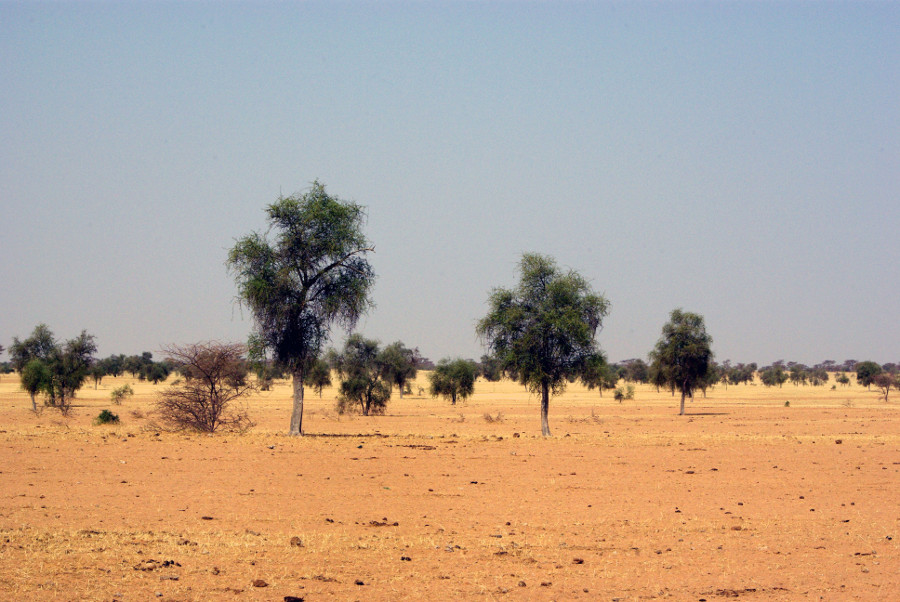
\includegraphics[width = 0.5\textwidth]{img/2007_Podor.JPG}
	\caption{FutureSahel Work Packages}
\end{figure}
\end{frame}

%-=-=-=-=-=-=-=-=-=-=-=-=-=-=-=-=-=-=-=-=-=-=-=-=
%	FRAME: Résilience et stockolm
%-=-=-=-=-=-=-=-=-=-=-=-=-=-=-=-=-=-=-=-=-=-=-=-=
\begin{frame}[c]{La résilience socio-environnementale : approche pratique}
\vspace{-1cm}
Peut-on considérer les services éco-systémiques rendus par l'arbre en contexte sahélien comme
facteur de résilience pour les populations et l'environnement?

L'OHM Téssékéré et l'ANR "future Sahel" travaillent avec le \textit{Stockholm Resilience Centre} sur l'application des concepts de résilience socio-environnementale à la zone de la grande muraille.

\begin{figure}
	\centering
	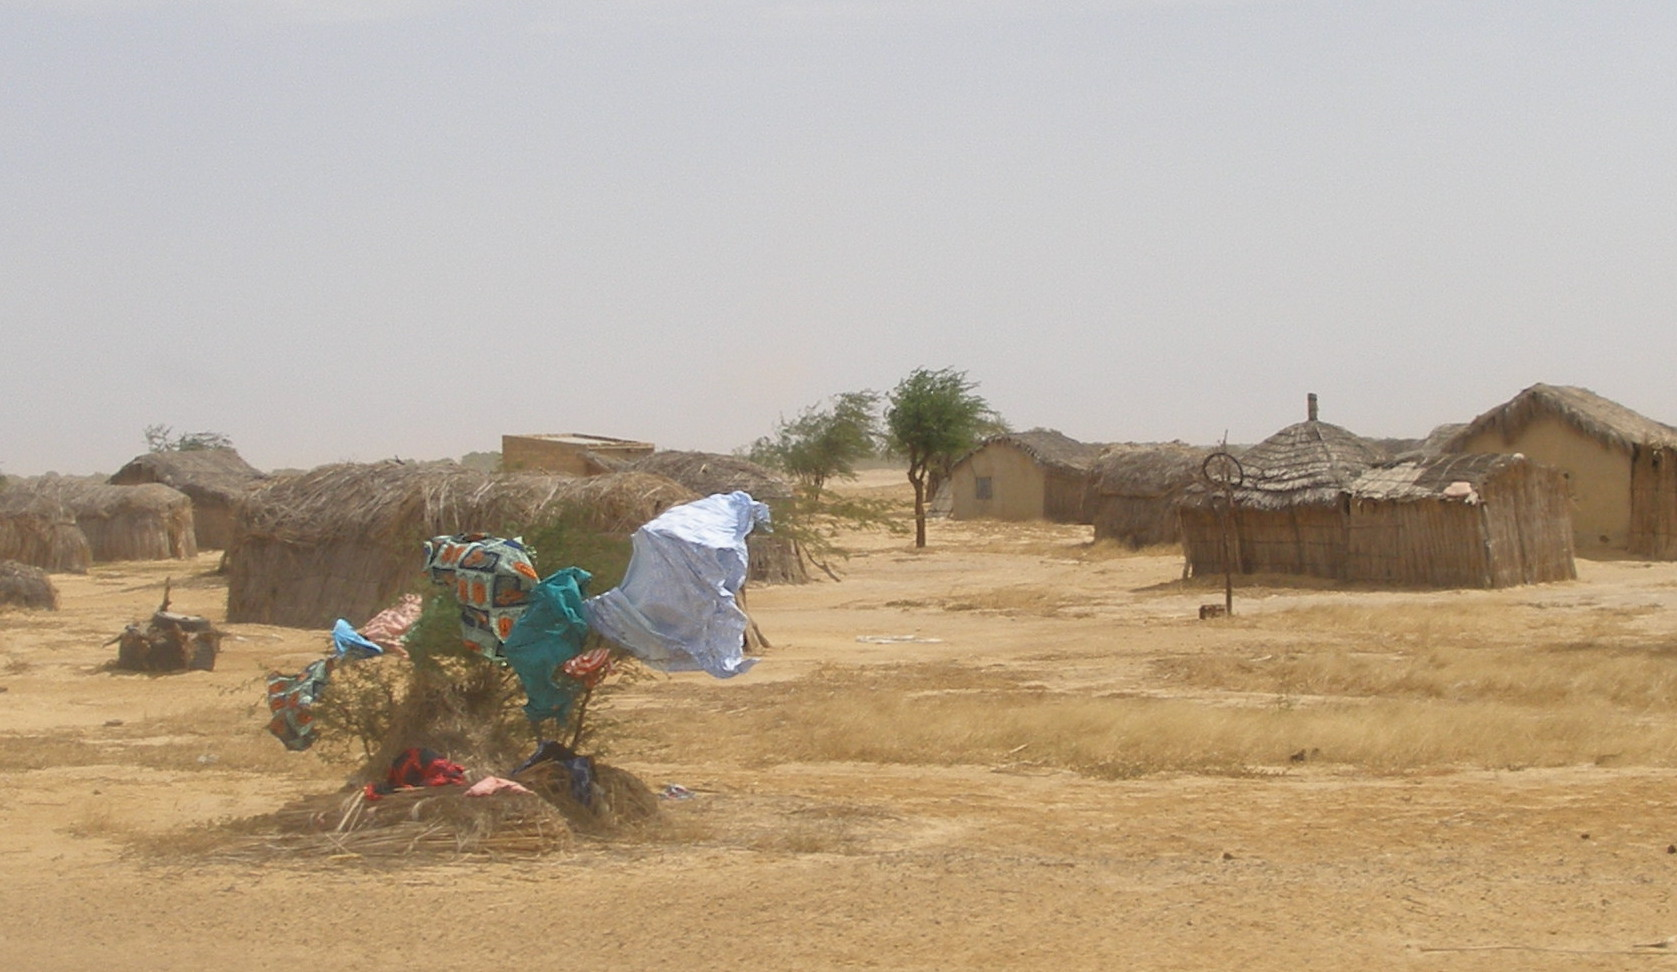
\includegraphics[width = 0.65\textwidth]{img/PA310152.JPG}
	\caption{FutureSahel Work Packages}
\end{figure}
\end{frame}


\section{methodologie - l'entree ethno-botanique}

%-=-=-=-=-=-=-=-=-=-=-=-=-=-=-=-=-=-=-=-=-=-=-=-=
%	FRAME: ethnobotanique
%-=-=-=-=-=-=-=-=-=-=-=-=-=-=-=-=-=-=-=-=-=-=-=-=
\begin{frame}[c]{Les entretiens ethnobotaniques}
\vspace{-1cm}

Entretiens semi-directifs structurés avec les acteurs (individuels et \textit{focus groups}) afin de comprendre la problématique et les réalités du terrain, de cerner les éléments essentiels à prendre en compte.

Connaître les usages, les stratégies de collecte, la saisonnalité, les modes de valorisation.

%Les entretiens se font en wolof et/ou poulard et son mener par plusieurs personnes en simultané sur les campements. Un brefing est réaliser au préalable pour explicier le guide d'entretien.

%acteurs photos jean-luc
\begin{figure}
	\centering
	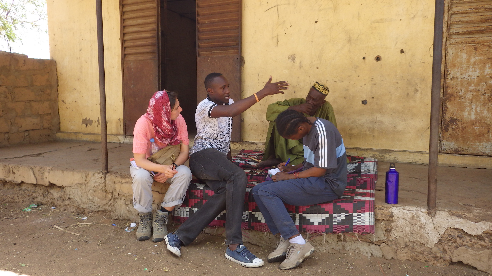
\includegraphics[height = 3.5cm]{img/group3.png}~
  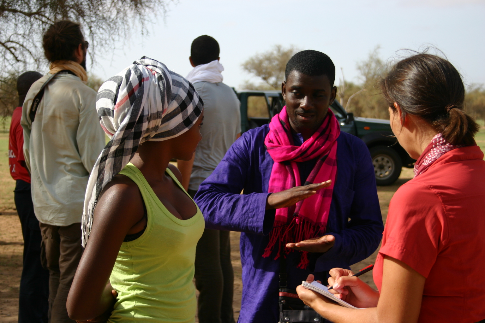
\includegraphics[height = 3.5cm]{img/group2.png}
\end{figure}
\end{frame}

%-=-=-=-=-=-=-=-=-=-=-=-=-=-=-=-=-=-=-=-=-=-=-=-=
%	FRAME: Questionnaires
%-=-=-=-=-=-=-=-=-=-=-=-=-=-=-=-=-=-=-=-=-=-=-=-=
\begin{frame}[c]{L'approche par questionnaires}
\vspace{-1cm}
Un questionnaire spécifique est utilisé pour quantifier les informations déjà obtenues dans les entretiens.

Réalisation de 30-40 questionnaires par site (un total de 200 questionnaires pour l’ensemble des sites).
%Image googleEarth des fenetres
\begin{figure}
	\centering
	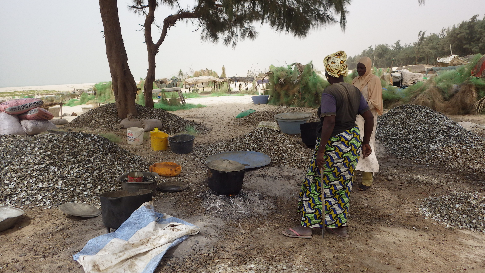
\includegraphics[width = 0.6\textwidth]{img/Khoudia.png}
\end{figure}

\end{frame}

%-=-=-=-=-=-=-=-=-=-=-=-=-=-=-=-=-=-=-=-=-=-=-=-=
%	FRAME: Ecologie du paysage
%-=-=-=-=-=-=-=-=-=-=-=-=-=-=-=-=-=-=-=-=-=-=-=-=
\section{methodologie - apports de l'ecologie du paysage}

\begin{frame}[c]{L'approche écologie du paysage 1/4}
\vspace{-1cm}
Un travail inspiré de la méthodologie proposée par Sinare \textit{et al.} (2016)
\begin{figure}
	\centering
	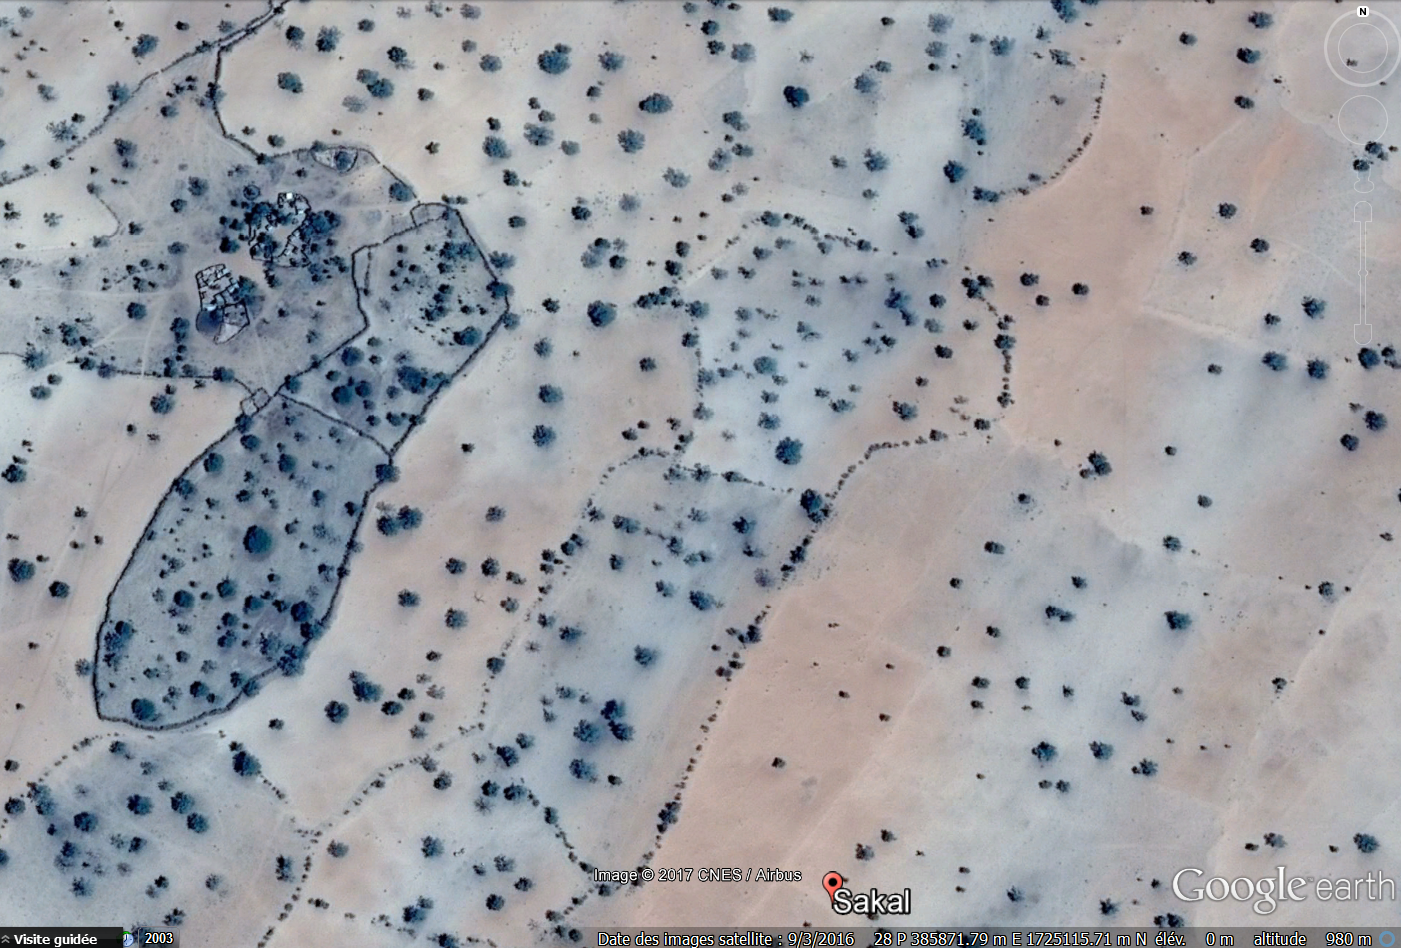
\includegraphics[height = 3.5cm]{img/ggearth}
  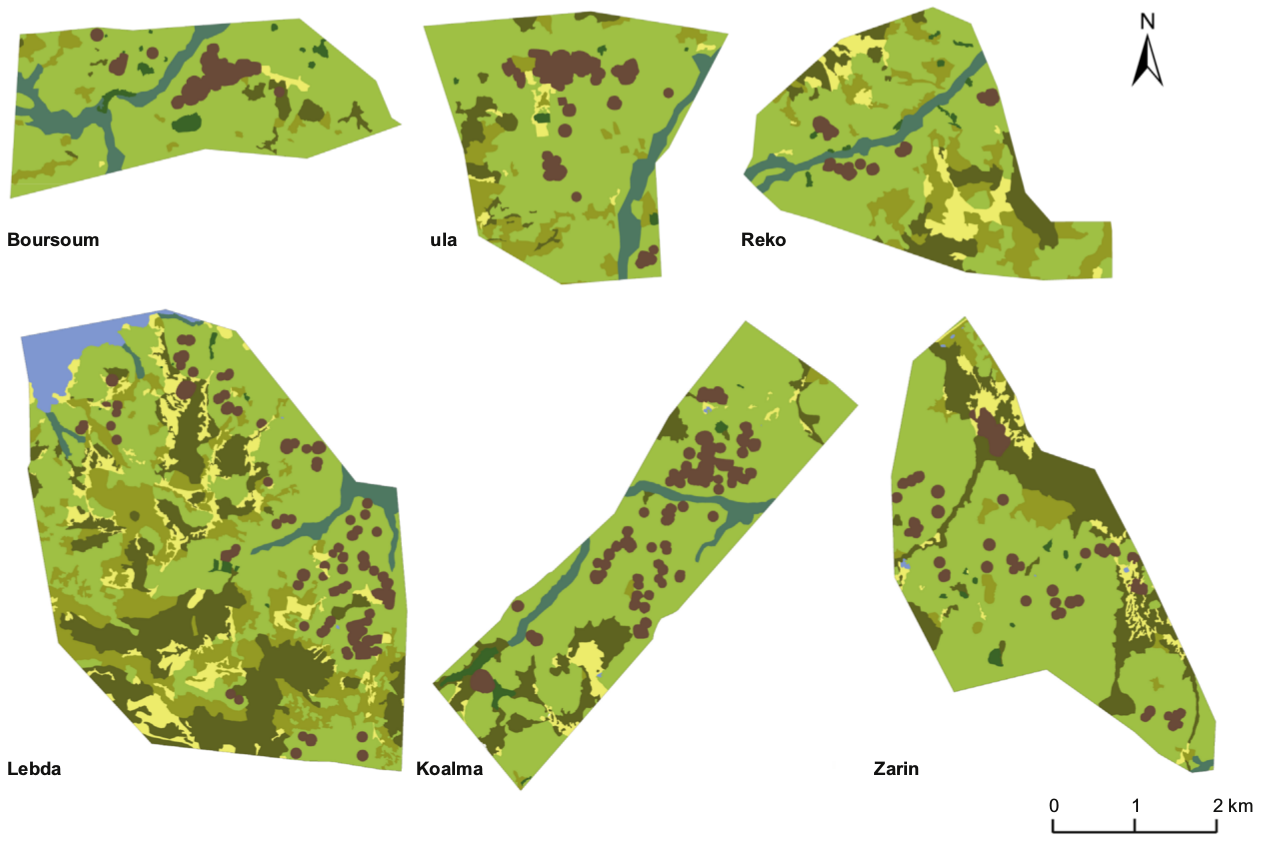
\includegraphics[height = 3.5cm]{img/Sinare_et_al2016}
  \caption{\small{Screenshot Google-earth and maps from Sinare \textit{et al.} (2016)}}
\end{figure}
\end{frame}

%-=-=-=-=-=-=-=-=-=-=-=-=-=-=-=-=-=-=-=-=-=-=-=-=
%	FRAME: Participation
%-=-=-=-=-=-=-=-=-=-=-=-=-=-=-=-=-=-=-=-=-=-=-=-=
\section{methodologie - la demarche participative}
\begin{frame}[c]{Les ateliers}
\vspace{-1cm}
Un travail en ateliers avec pour objectif de faire évaluer par les acteurs l'importance des arbres dans chaque structure du paysage.
\begin{itemize}
  \item structurer l'espace (orientation + repères de l'espace vecu),
  \item identifier les unités spatiales présentes,
  \item quantifier l'usage de l'arbre dans ces unités.
\end{itemize}
\begin{figure}
	\centering
	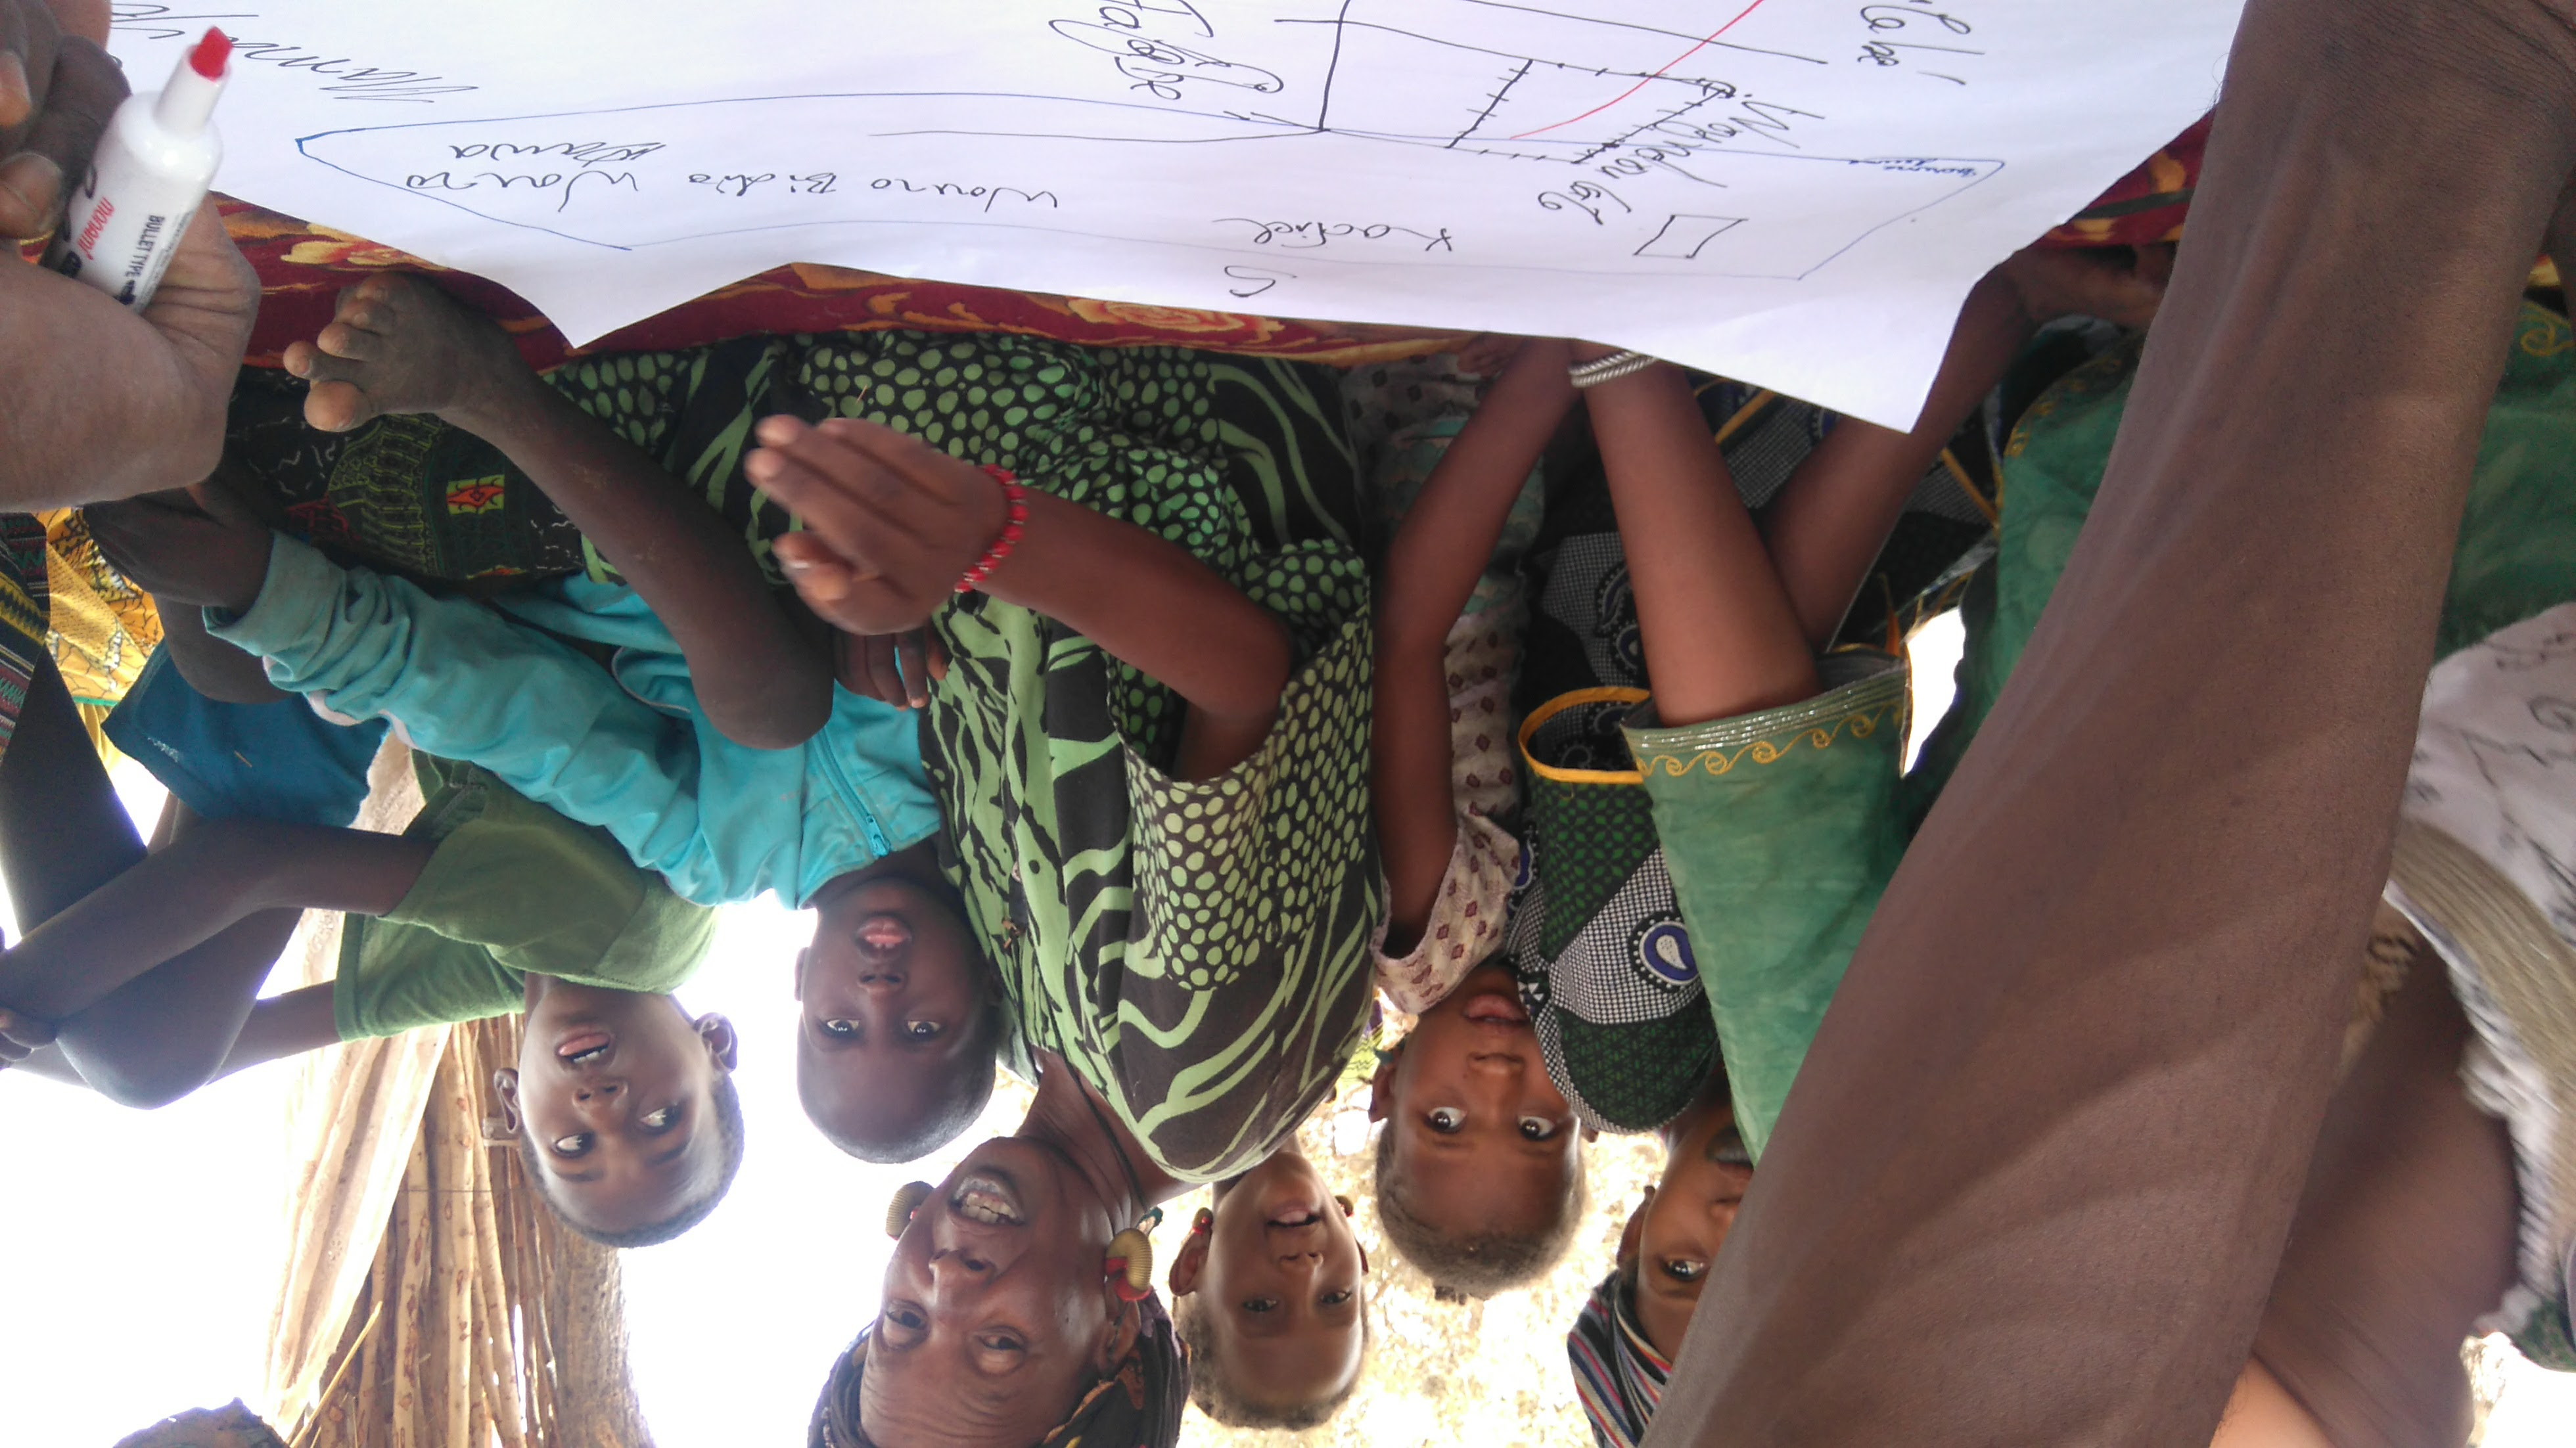
\includegraphics[width = 0.6\textwidth,angle=180]{img/DSC_1789}
\end{figure}
\end{frame}

%-=-=-=-=-=-=-=-=-=-=-=-=-=-=-=-=-=-=-=-=-=-=-=-=
%	FRAME: Unité paysagères
%-=-=-=-=-=-=-=-=-=-=-=-=-=-=-=-=-=-=-=-=-=-=-=-=

\begin{frame}[c]{Les ateliers et l'écologie du paysage 1/2}
\vspace{-1cm}
\begin{figure}
  \subfigure[]{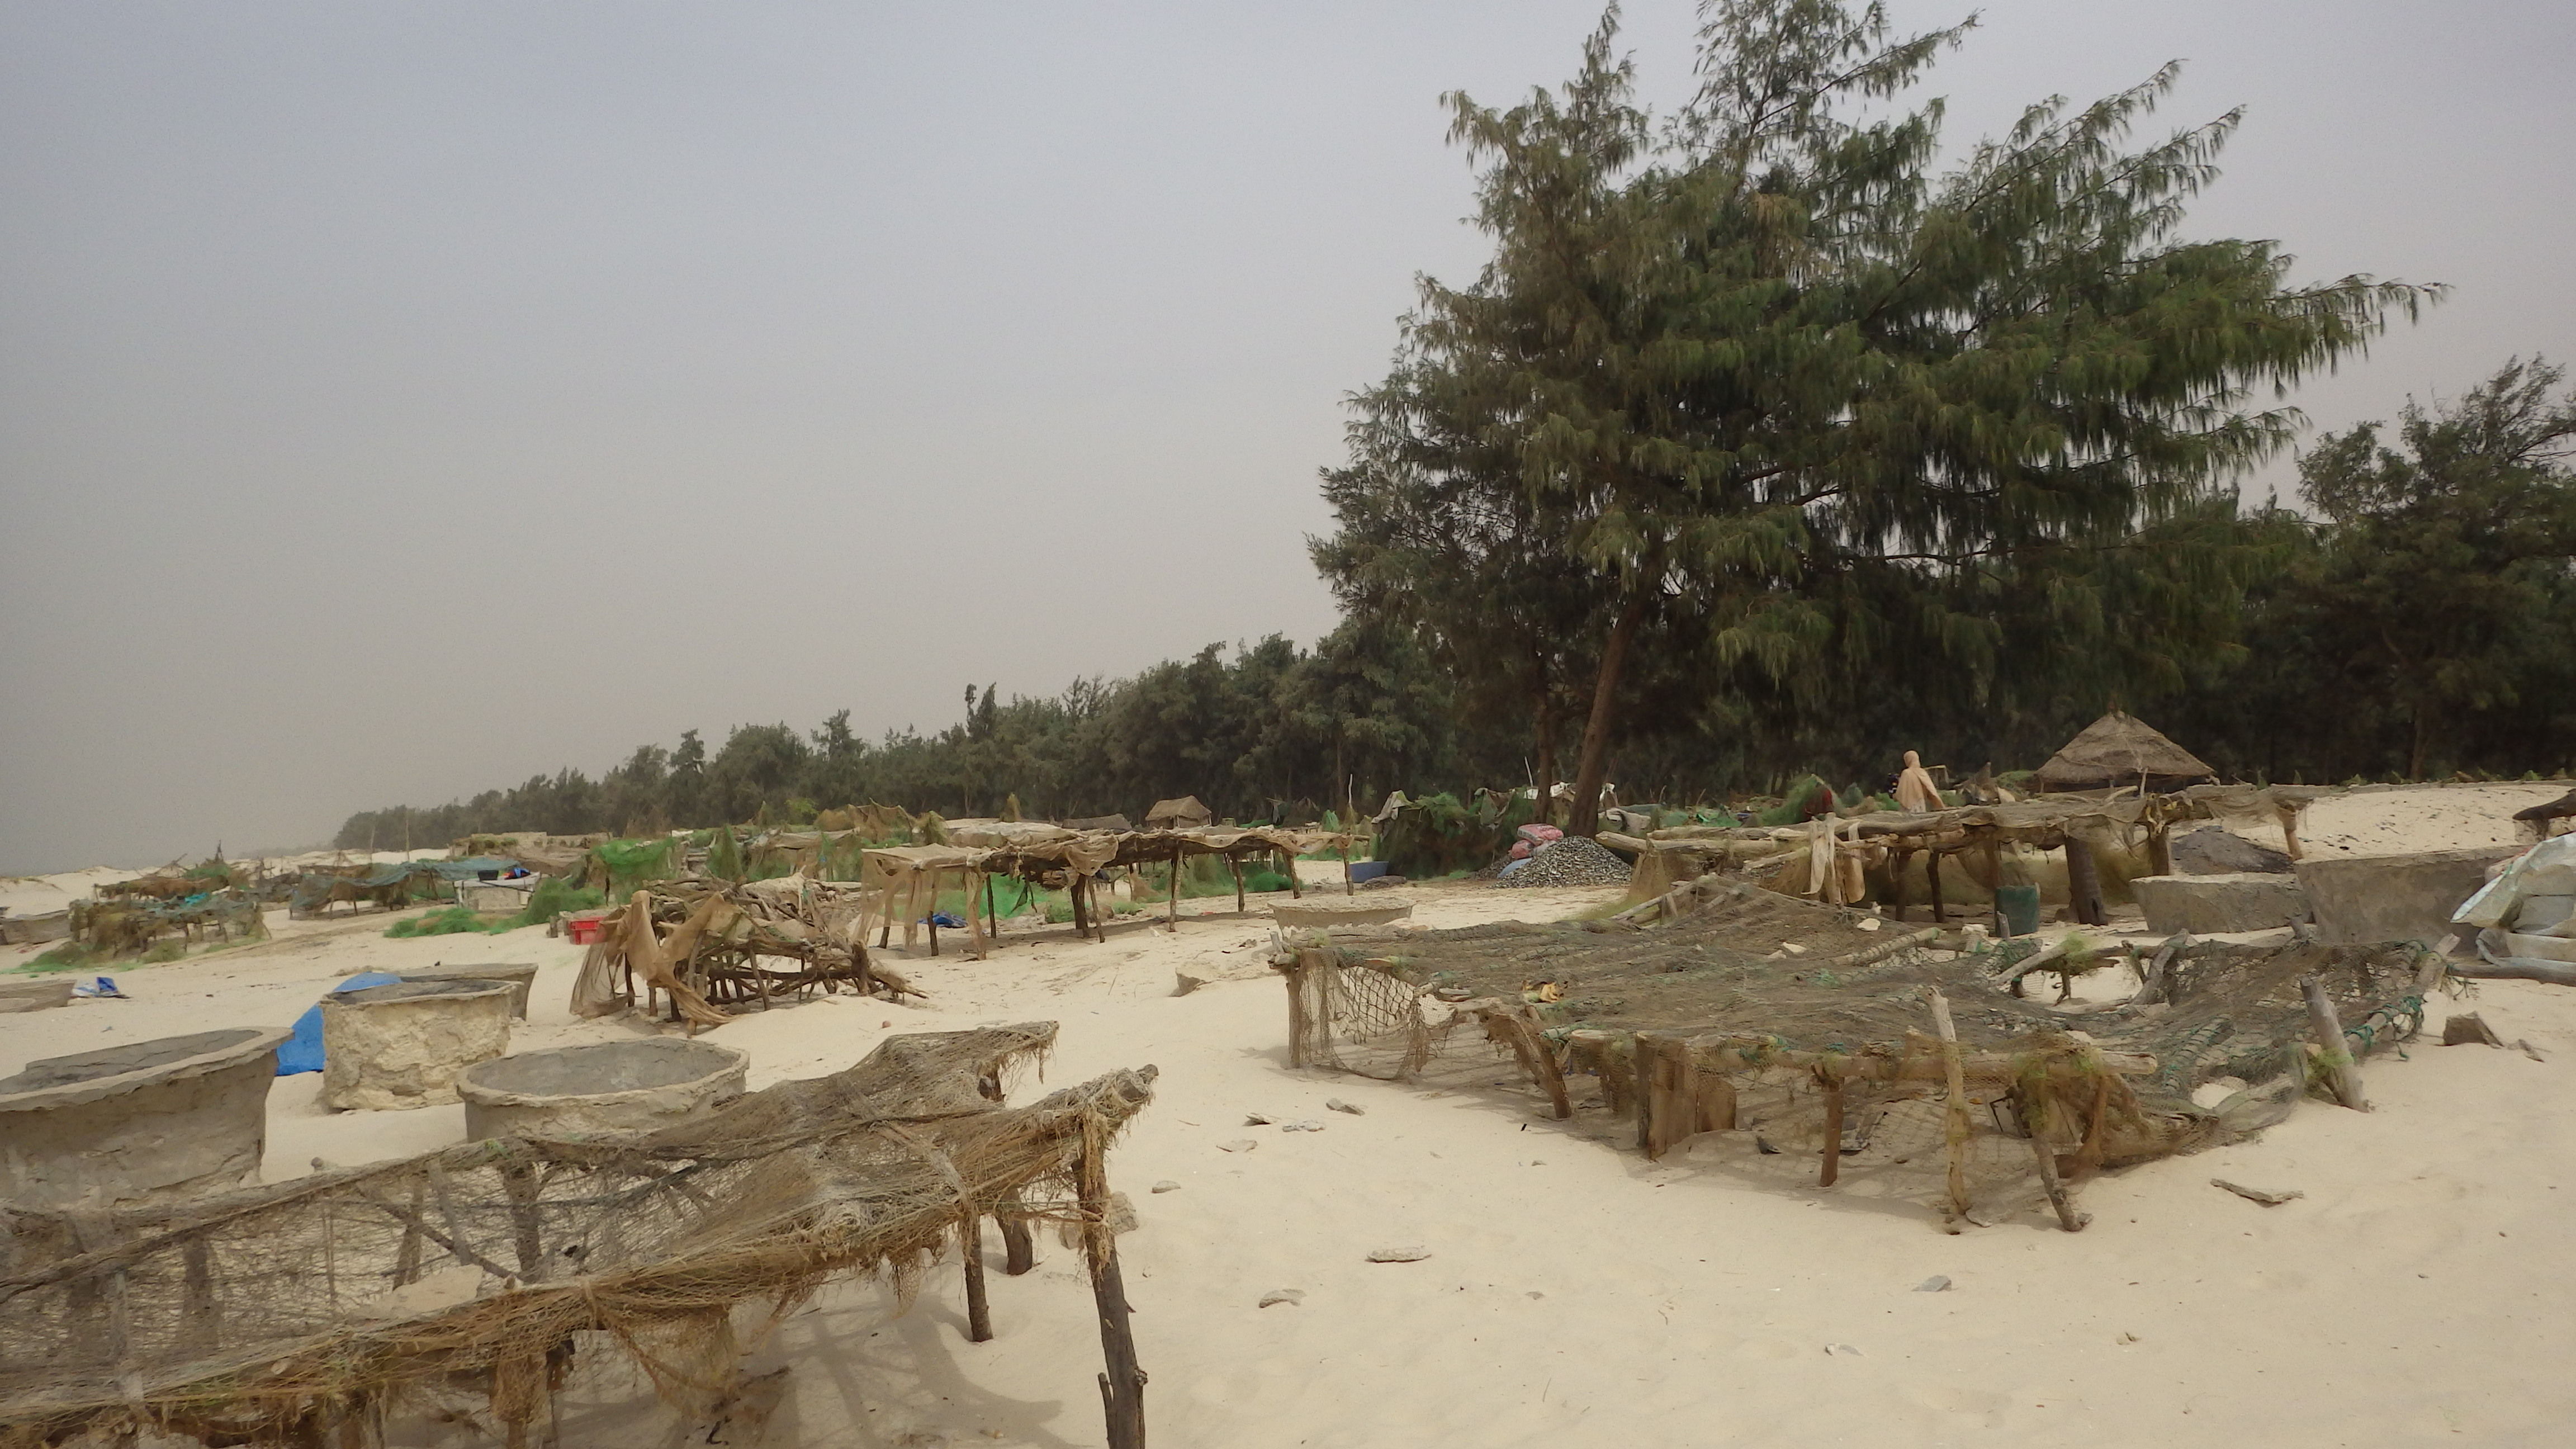
\includegraphics[height = 2.5cm]{img/photo_mission/01_Plage_filao}}
  \subfigure[]{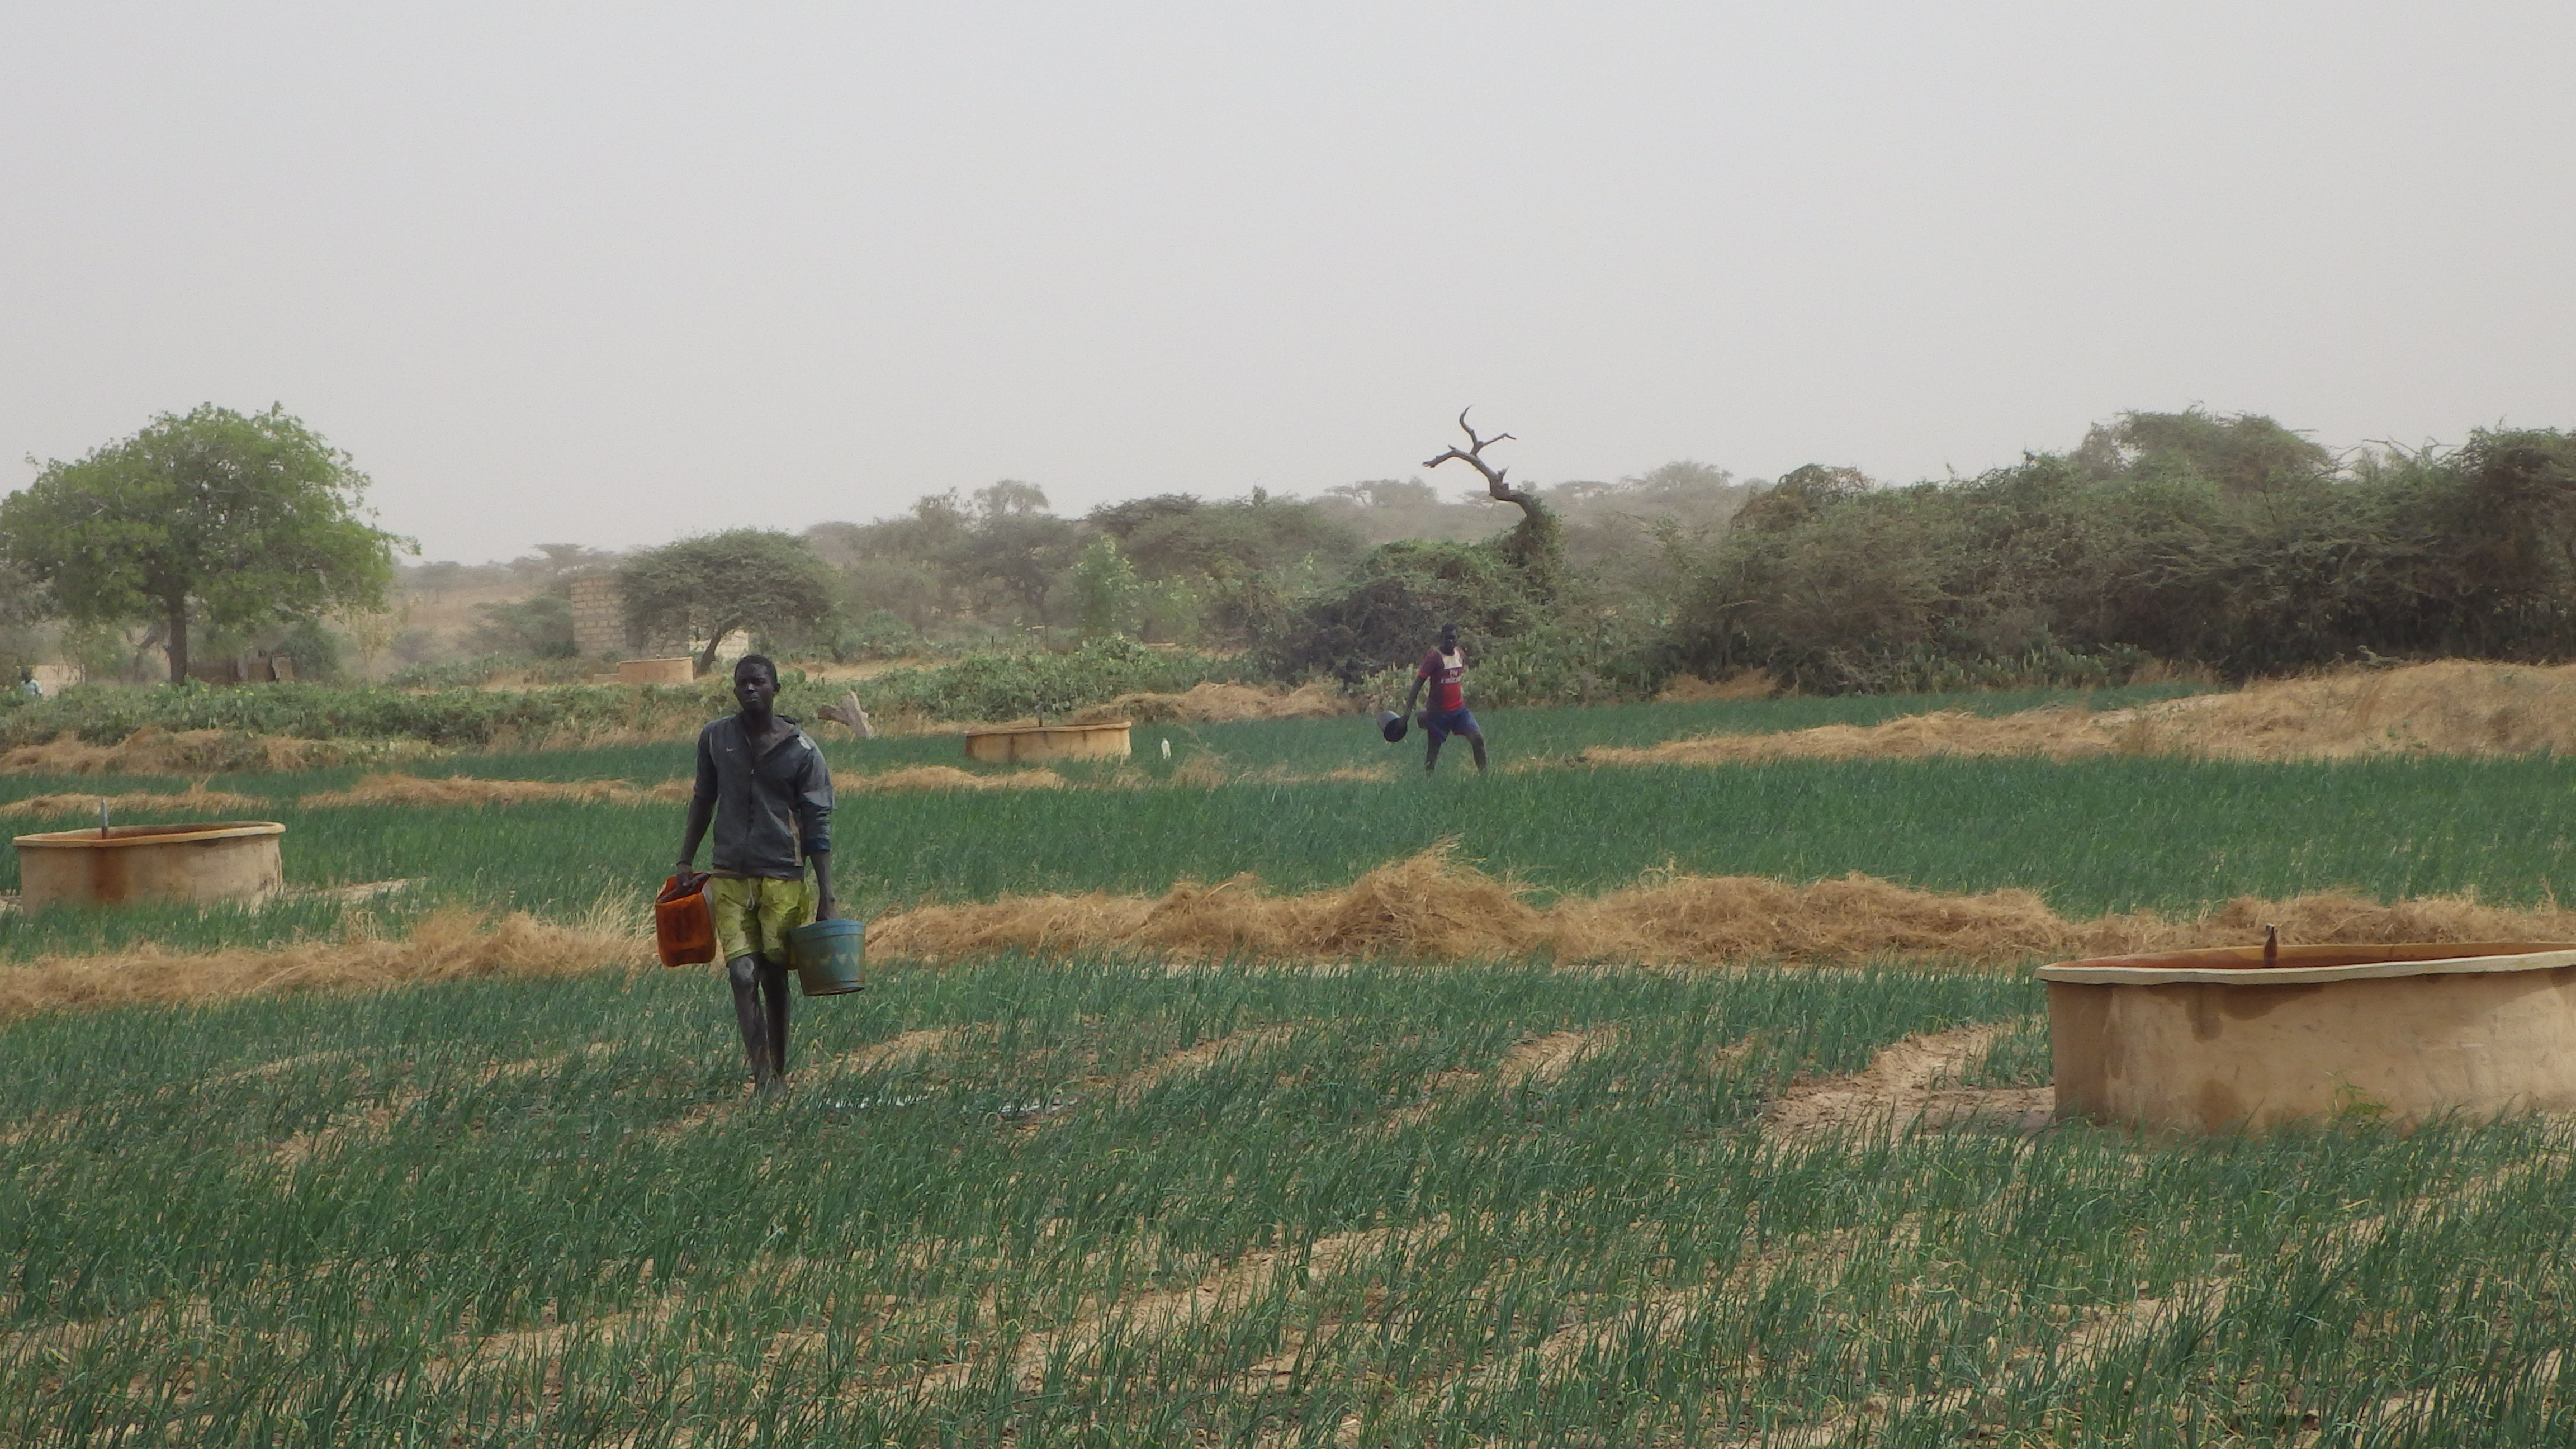
\includegraphics[height = 2.5cm]{img/photo_mission/02_Champs_irrigue}}\\
  \subfigure[]{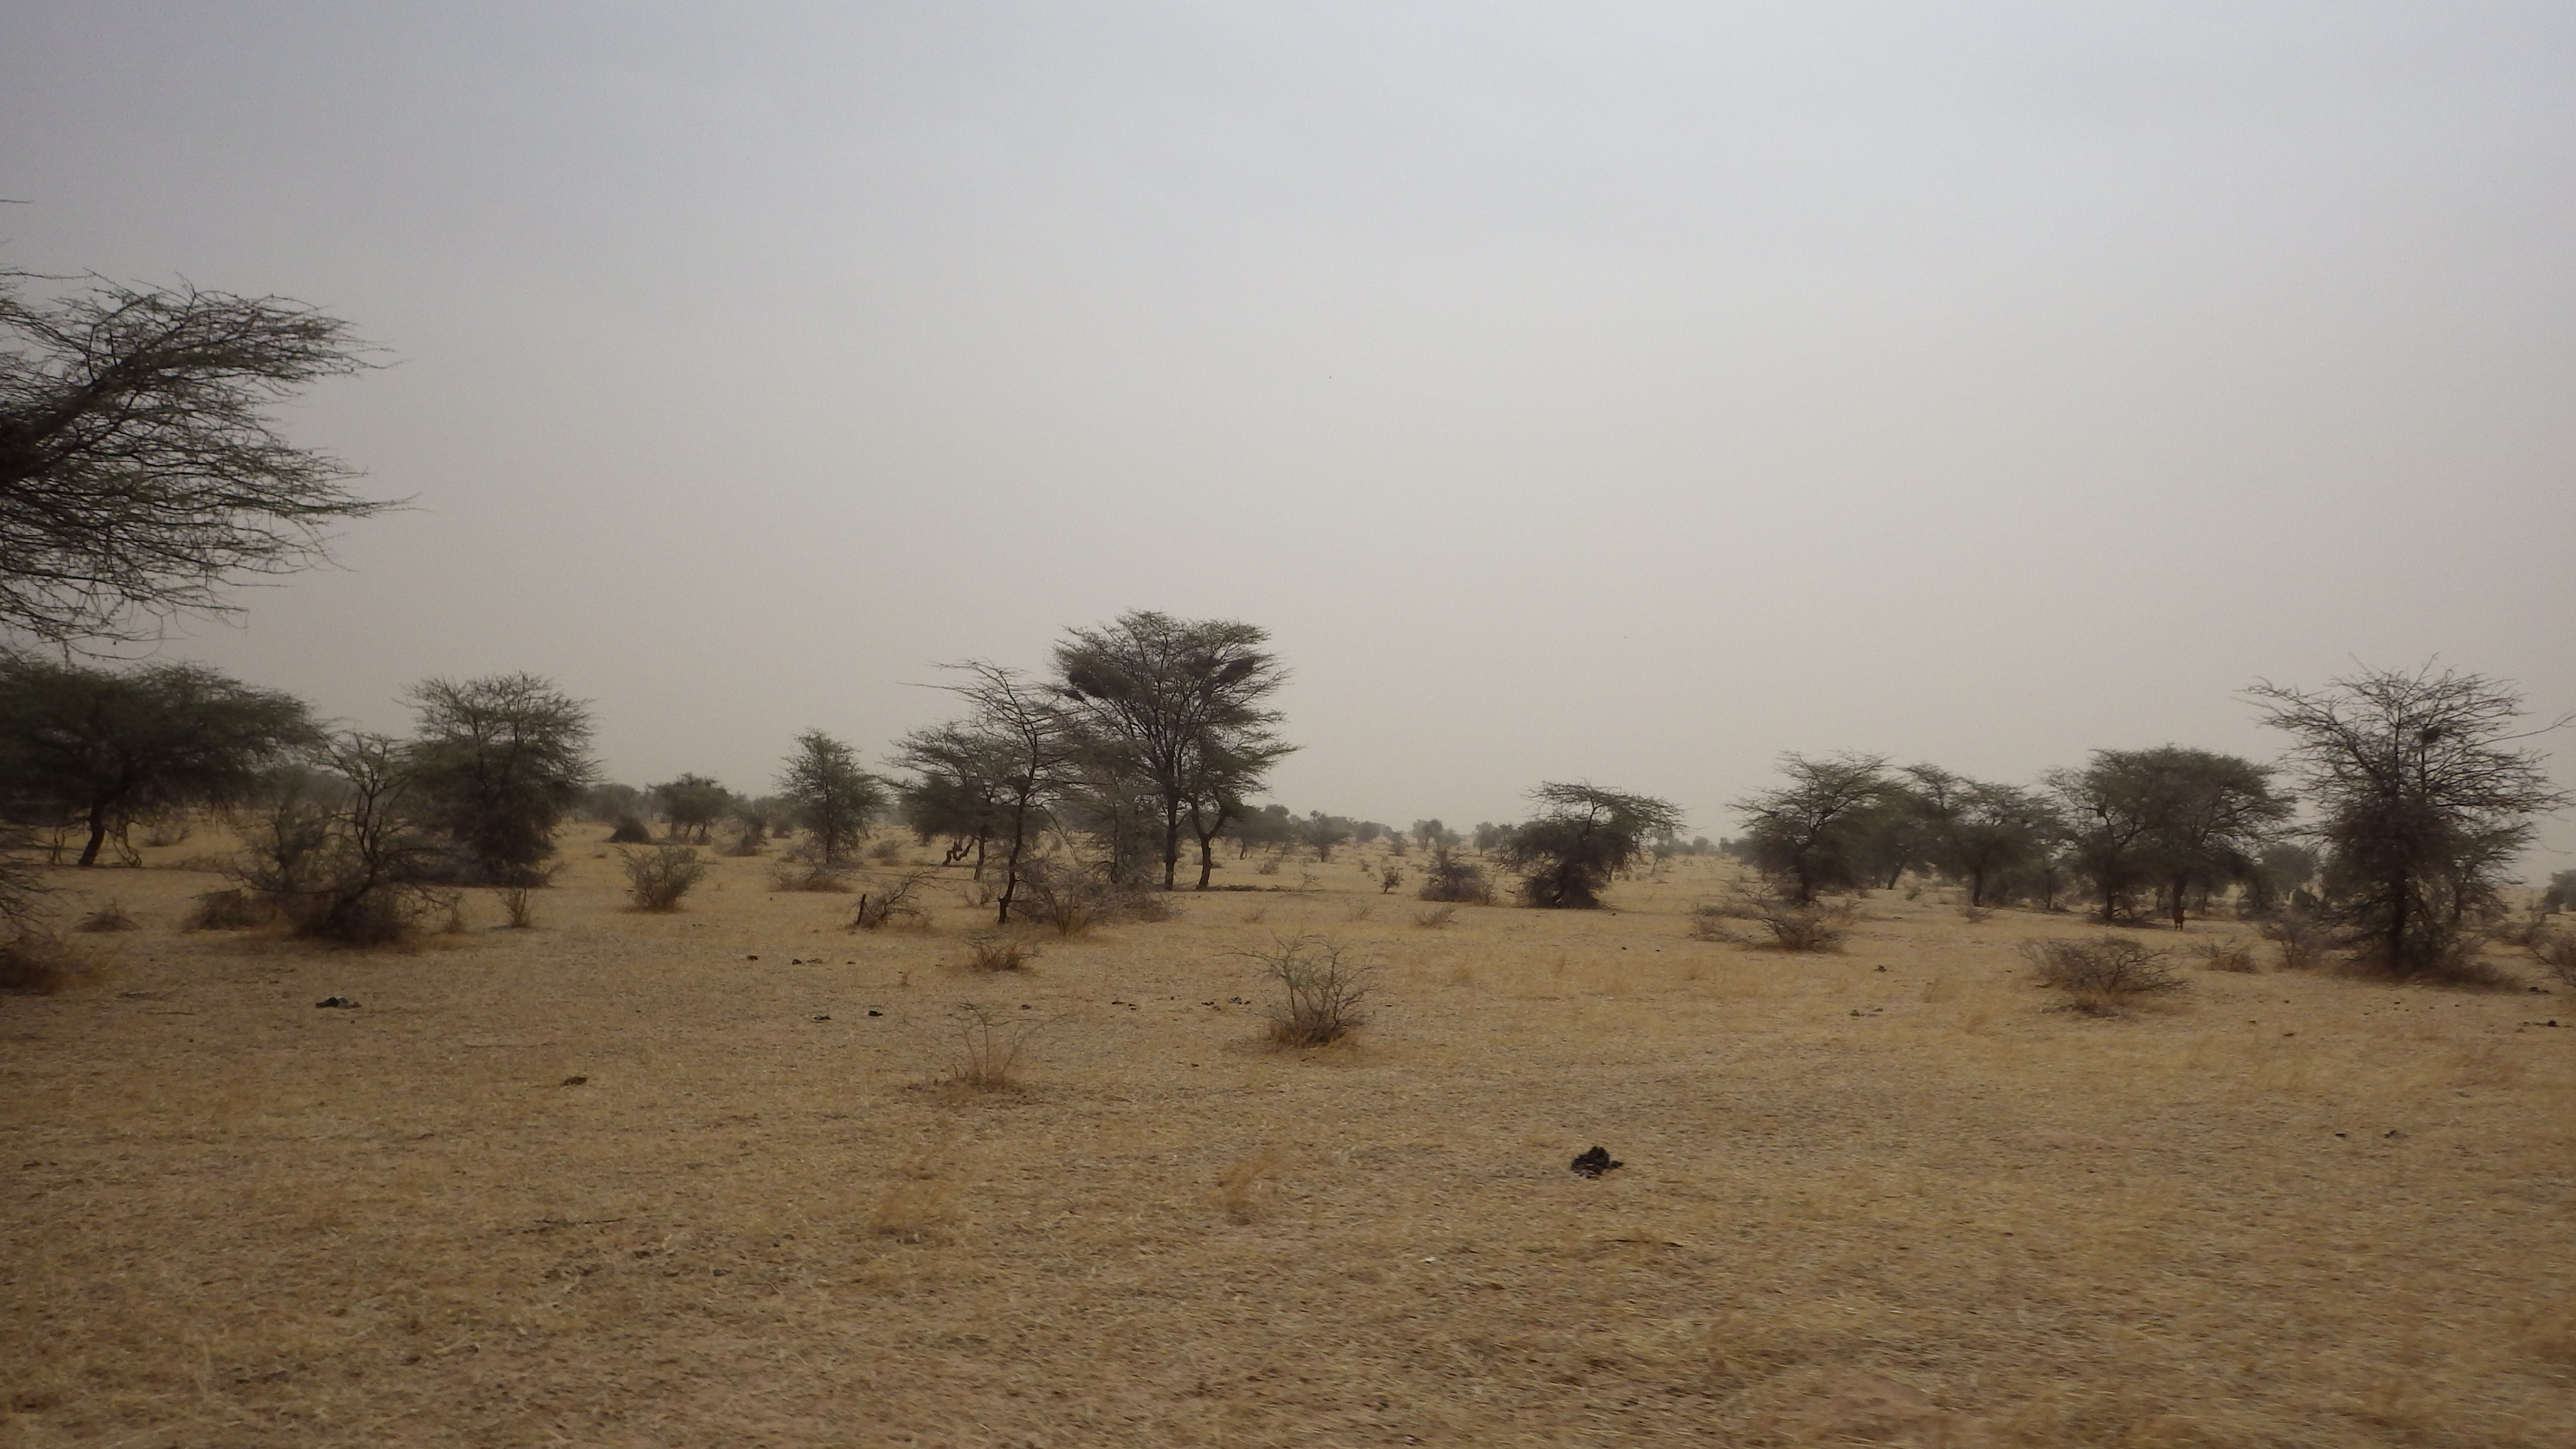
\includegraphics[height = 2.5cm]{img/photo_mission/03_Brousse_peu_dense}}
  \subfigure[]{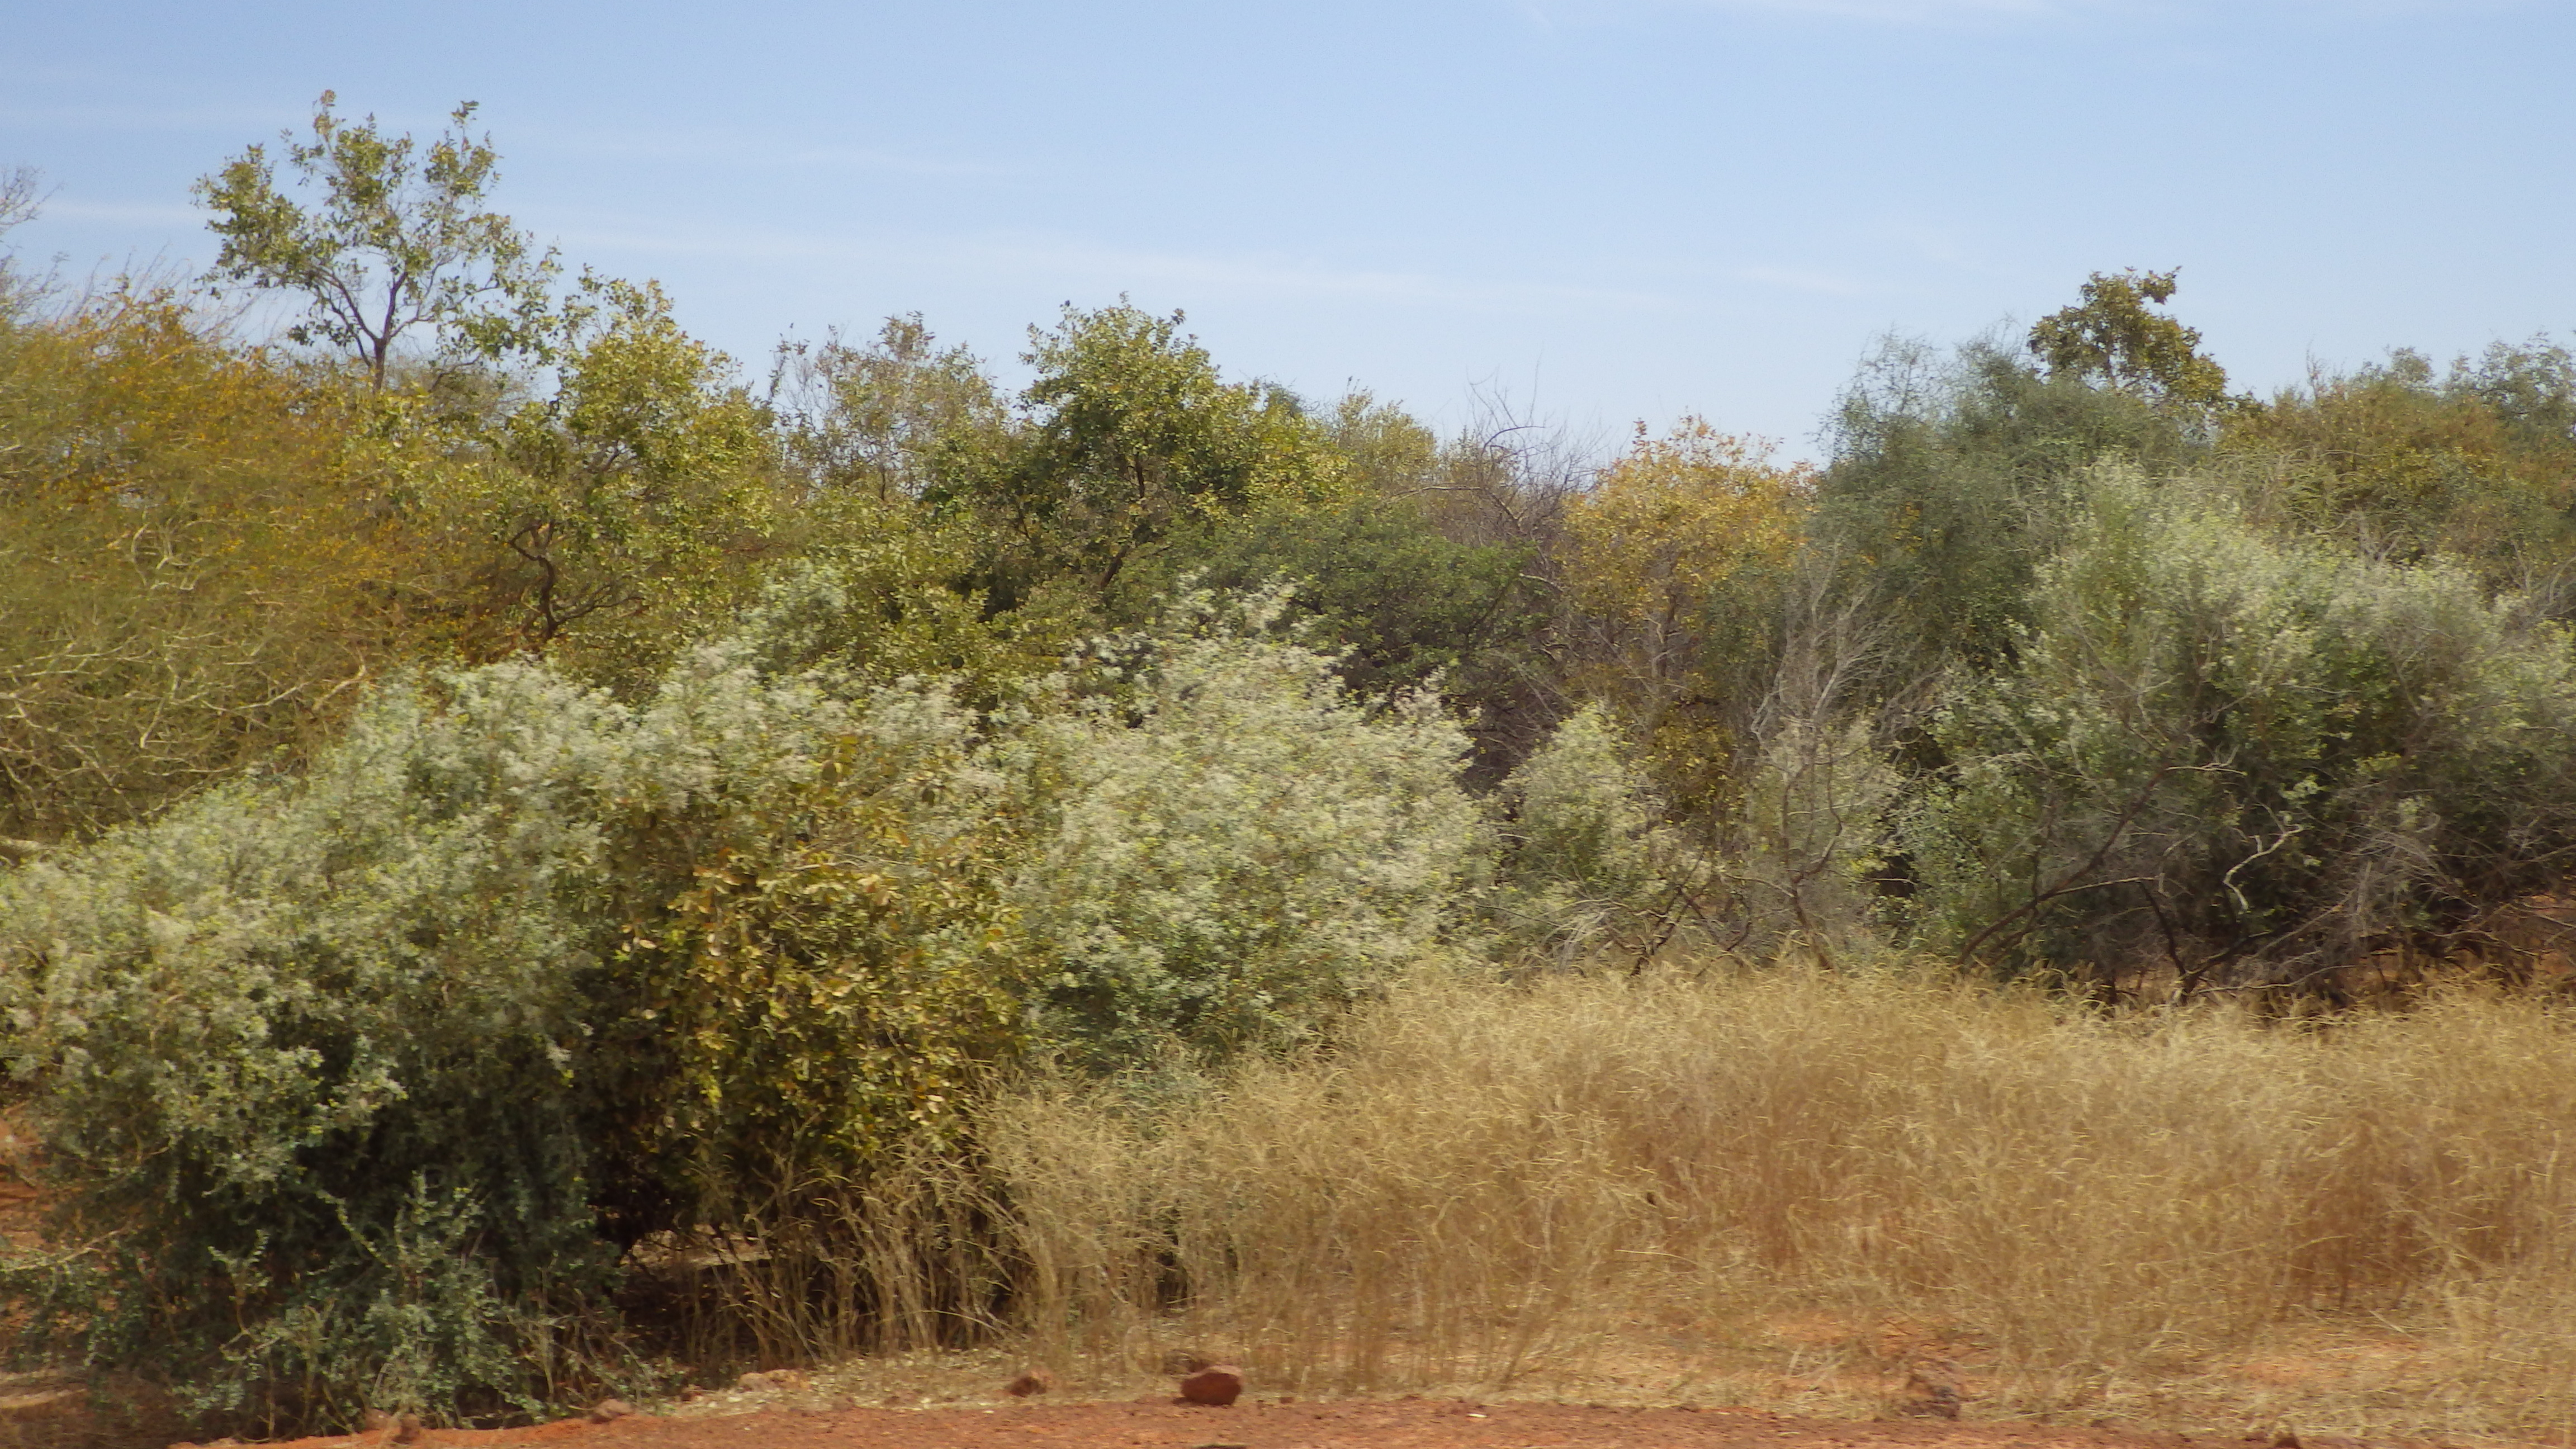
\includegraphics[height = 2.5cm]{img/photo_mission/05_Brousse_dense}}
\end{figure}

\end{frame}

\begin{frame}[c]{Les ateliers et l'écologie du paysage 2/2}
\vspace{-1cm}
\begin{figure}
	\subfigure[]{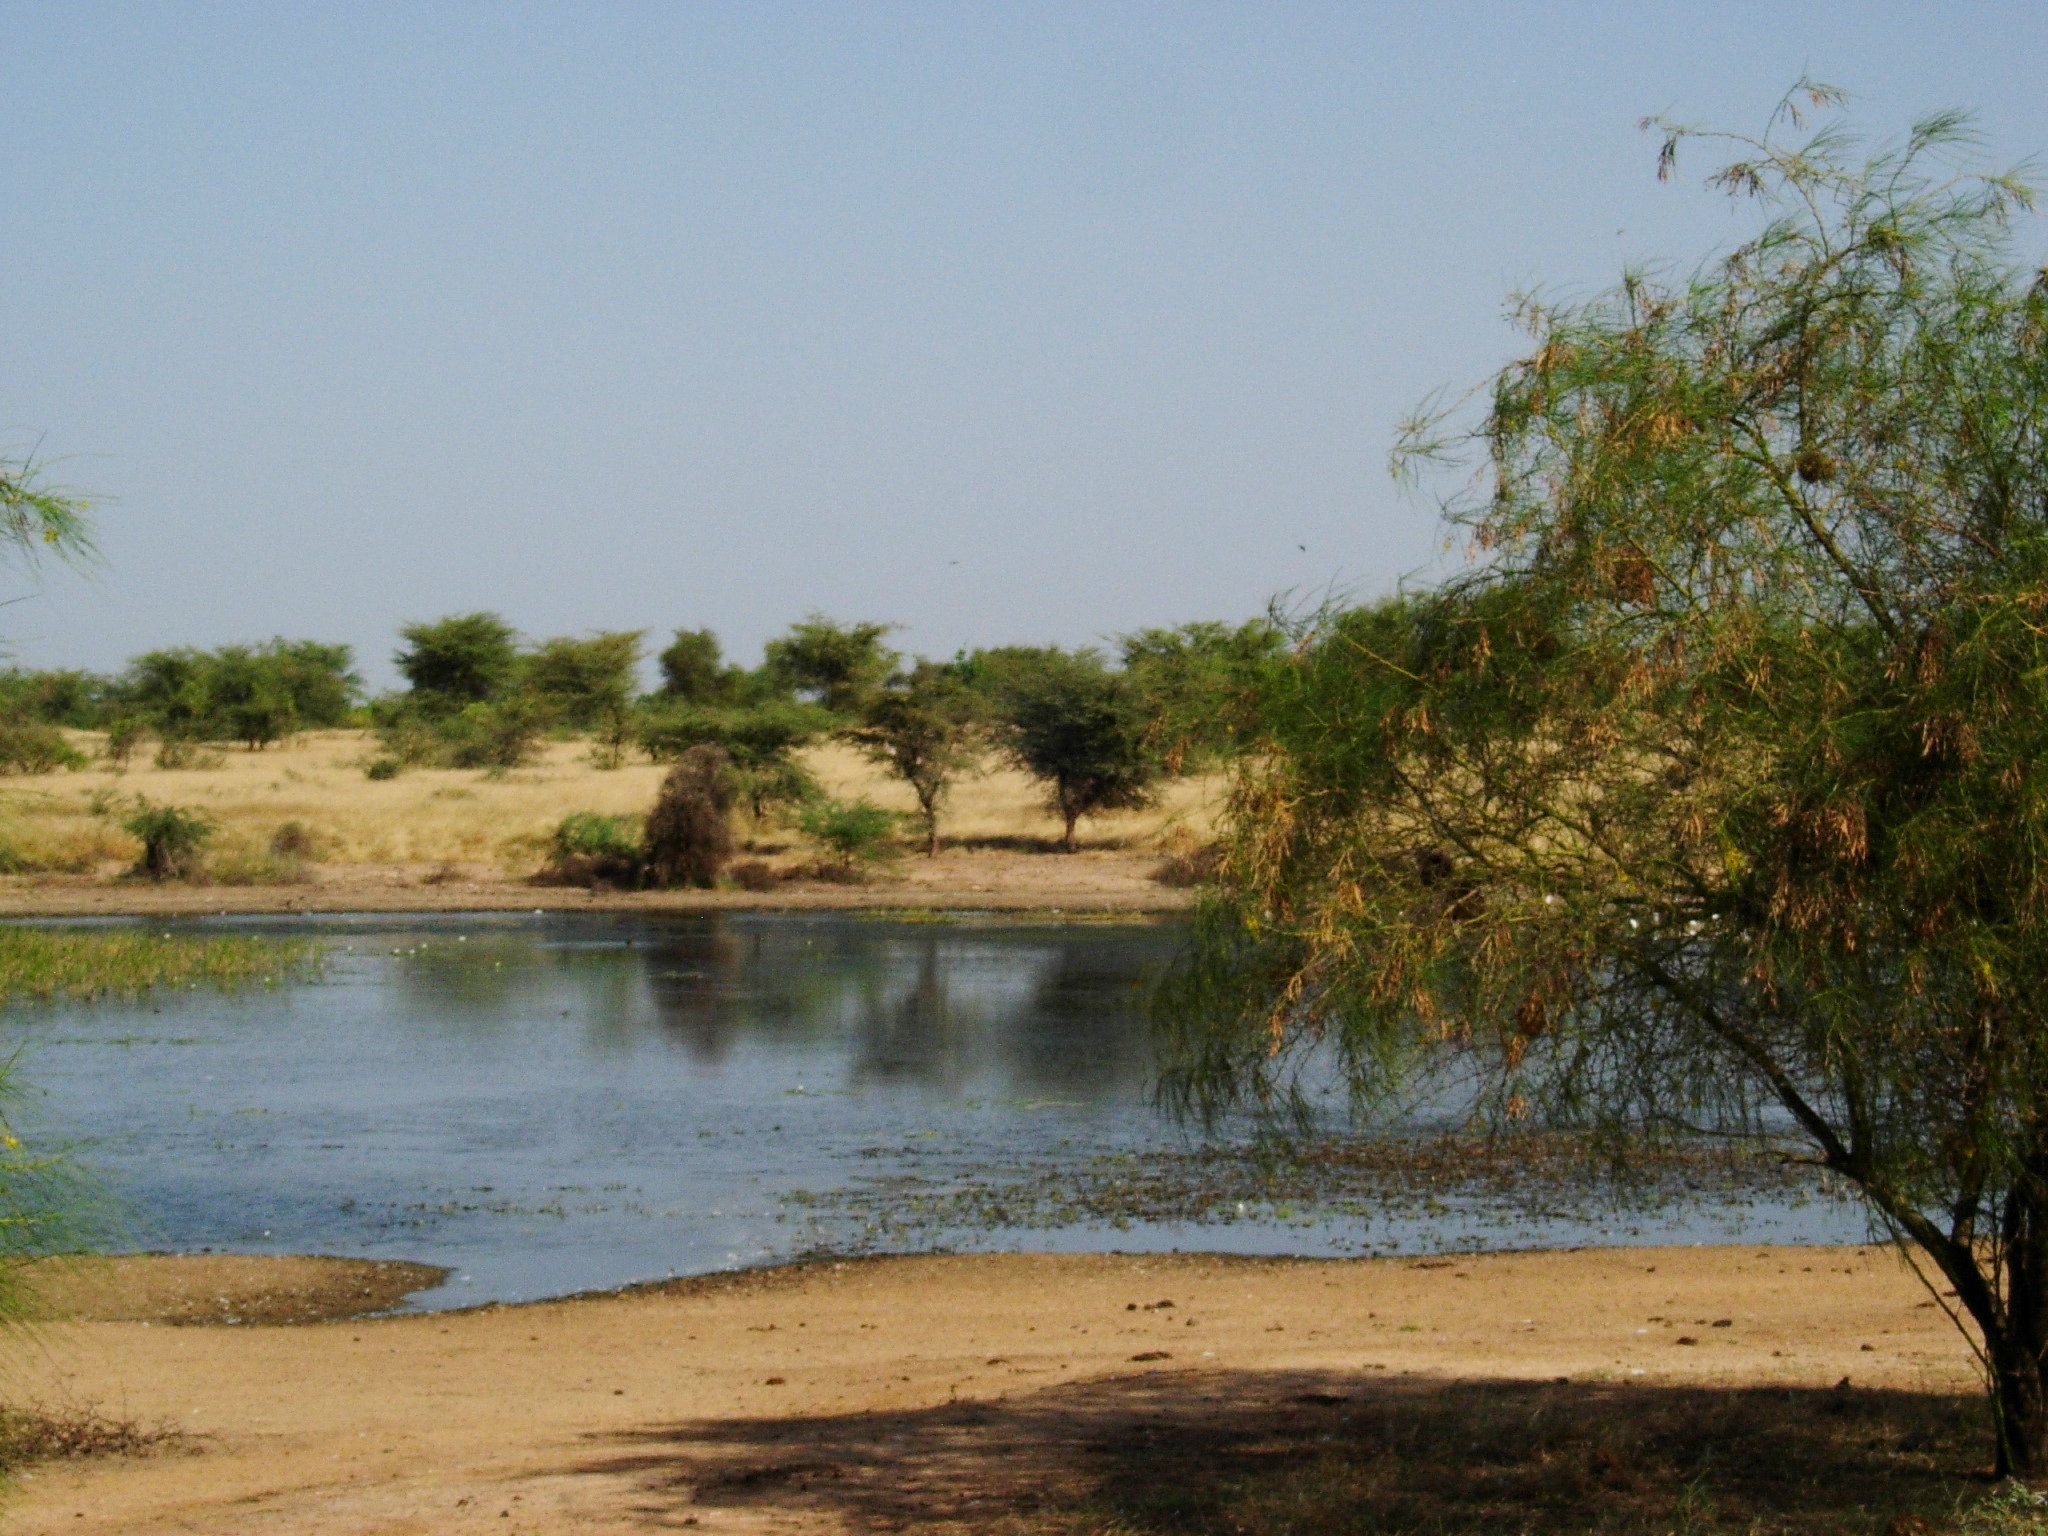
\includegraphics[height = 2.5cm]{img/photo_mission/06_Mares}}
  \subfigure[]{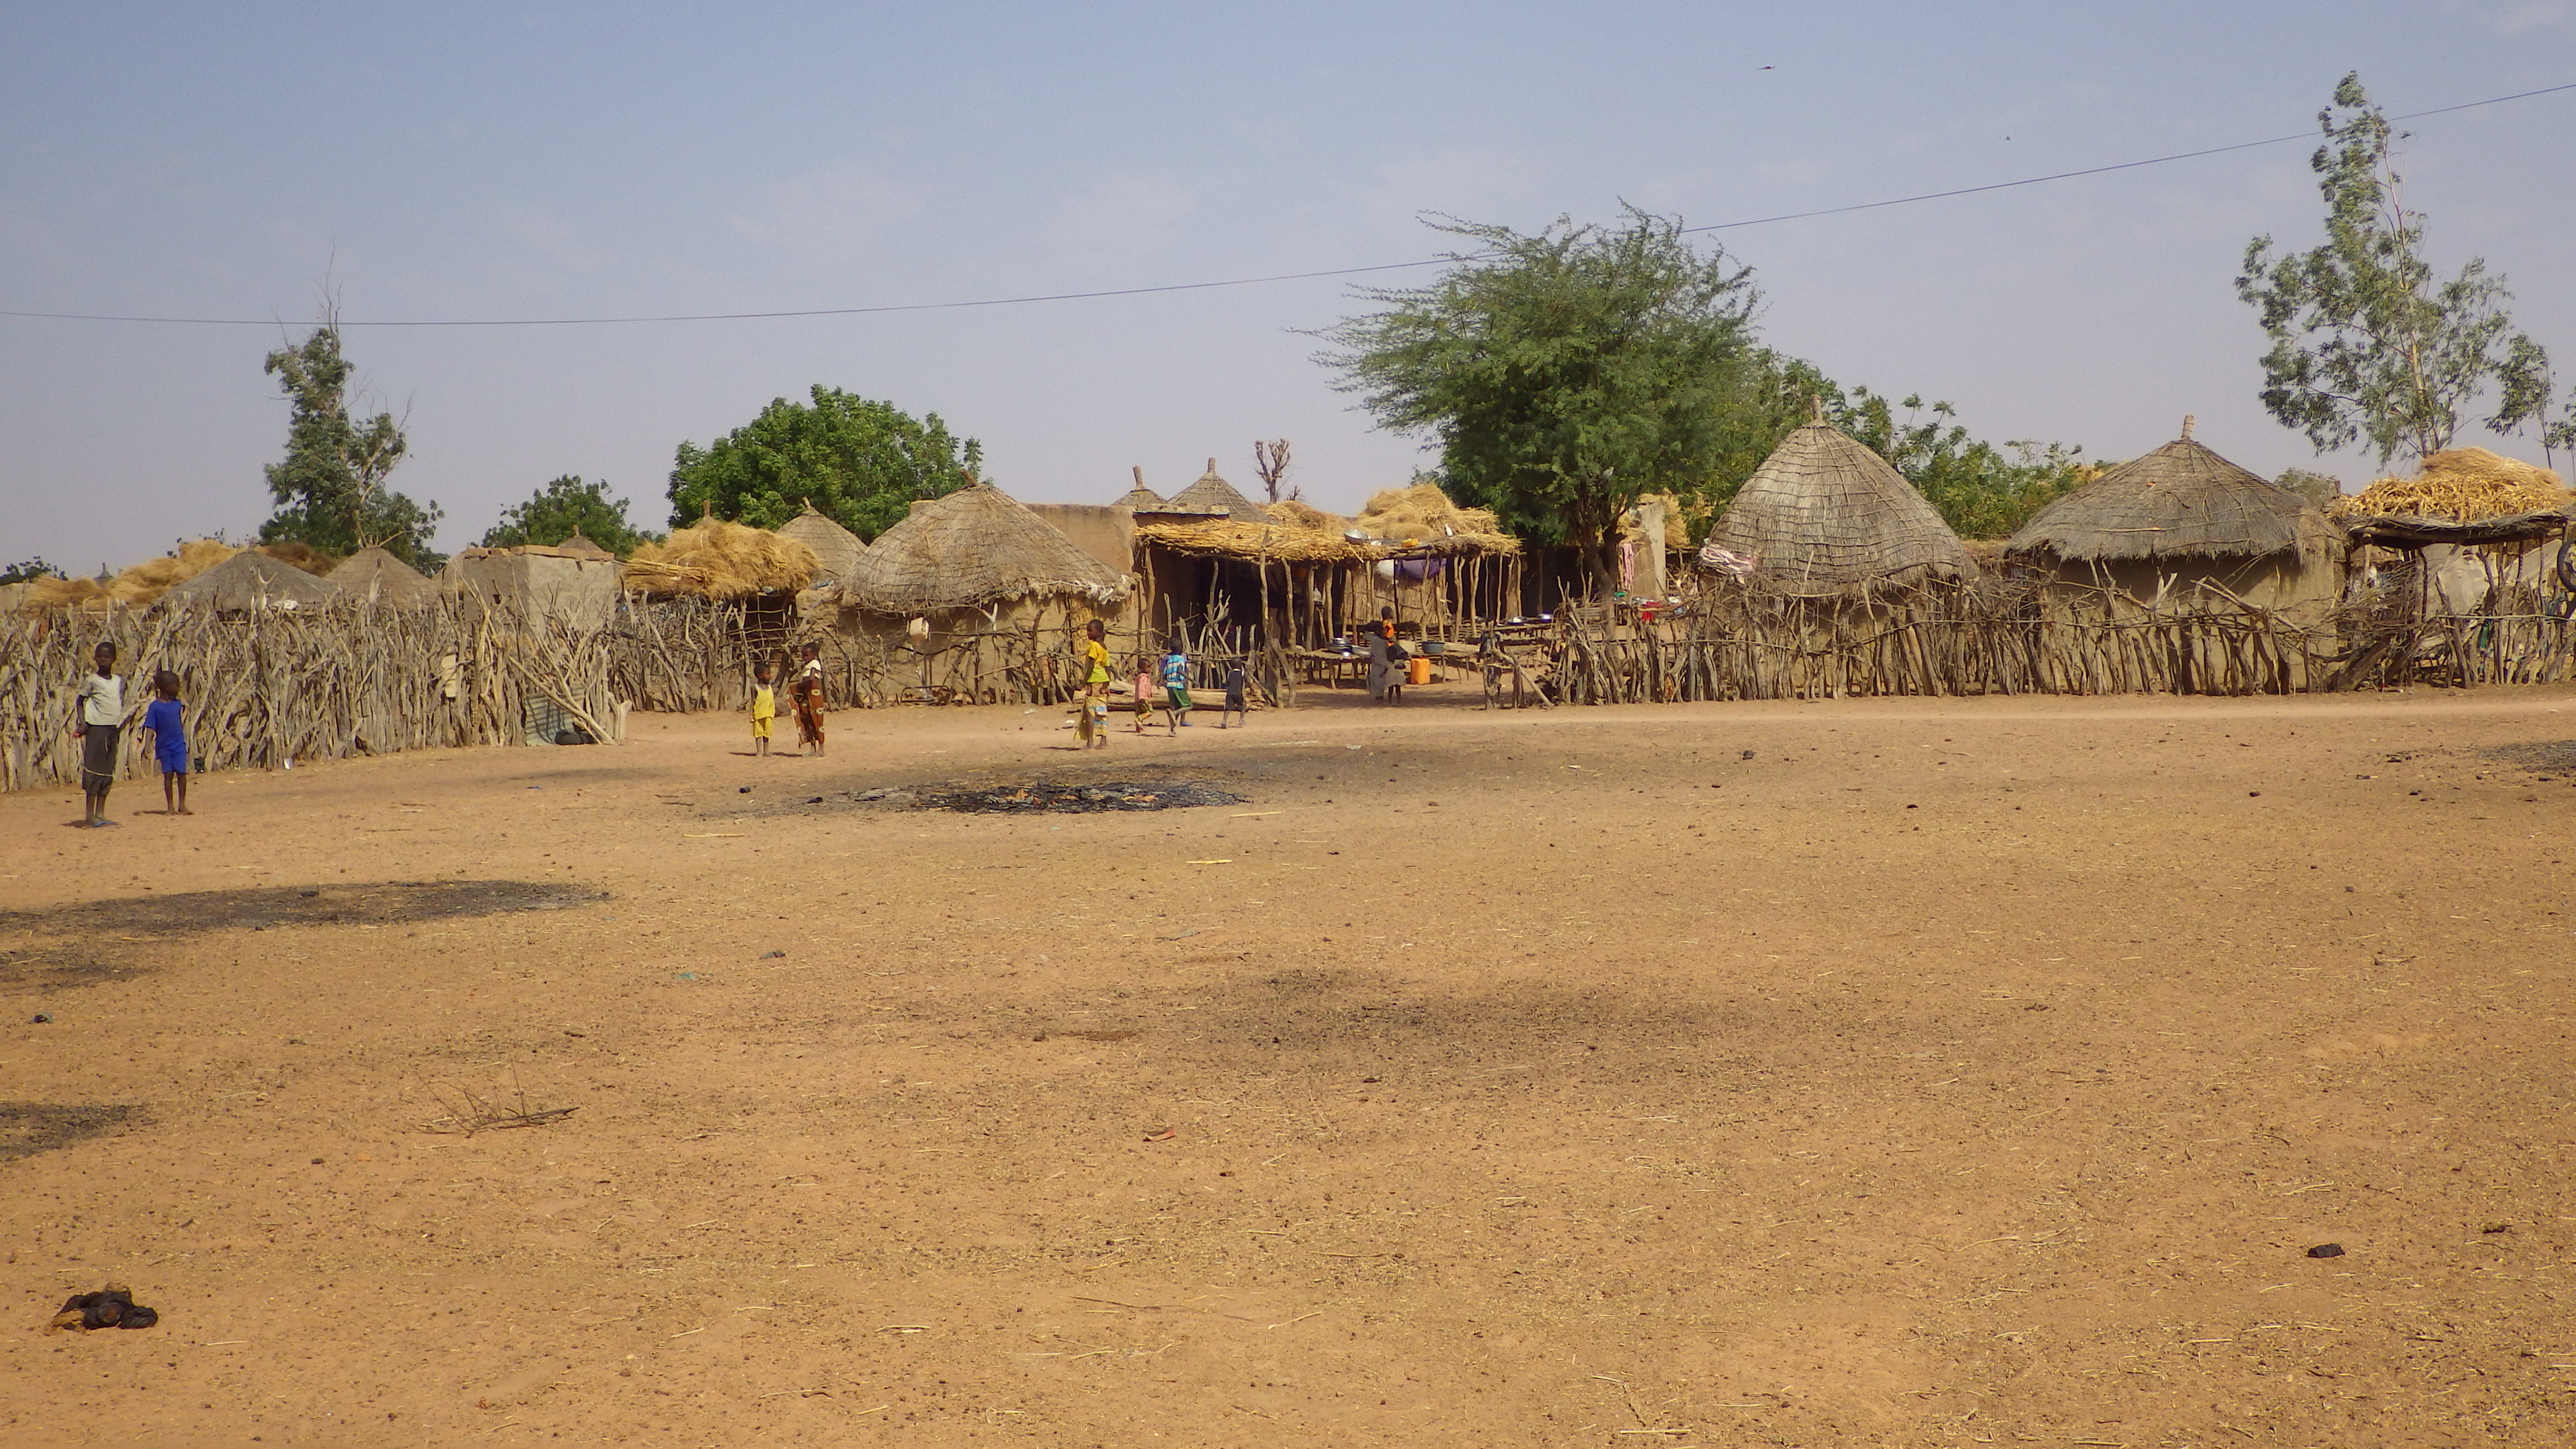
\includegraphics[height = 2.5cm]{img/photo_mission/07_Homestead}}\\
  \subfigure[]{\includegraphics[height = 2.5cm]{img/photo_mission/08_Agriculture_pluvial}}
  \subfigure[]{\includegraphics[height = 2.5cm]{img/photo_mission/10_Parcelle_reboisement}}
\end{figure}
\end{frame}

%-=-=-=-=-=-=-=-=-=-=-=-=-=-=-=-=-=-=-=-=-=-=-=-=
%	FRAME: Quantification
%-=-=-=-=-=-=-=-=-=-=-=-=-=-=-=-=-=-=-=-=-=-=-=-=

\begin{frame}[c]{Les ateliers et les usages}
\vspace{-1cm}
Quantifier les usages liés à l'arbre dans l'espace
\begin{figure}
  \centering
  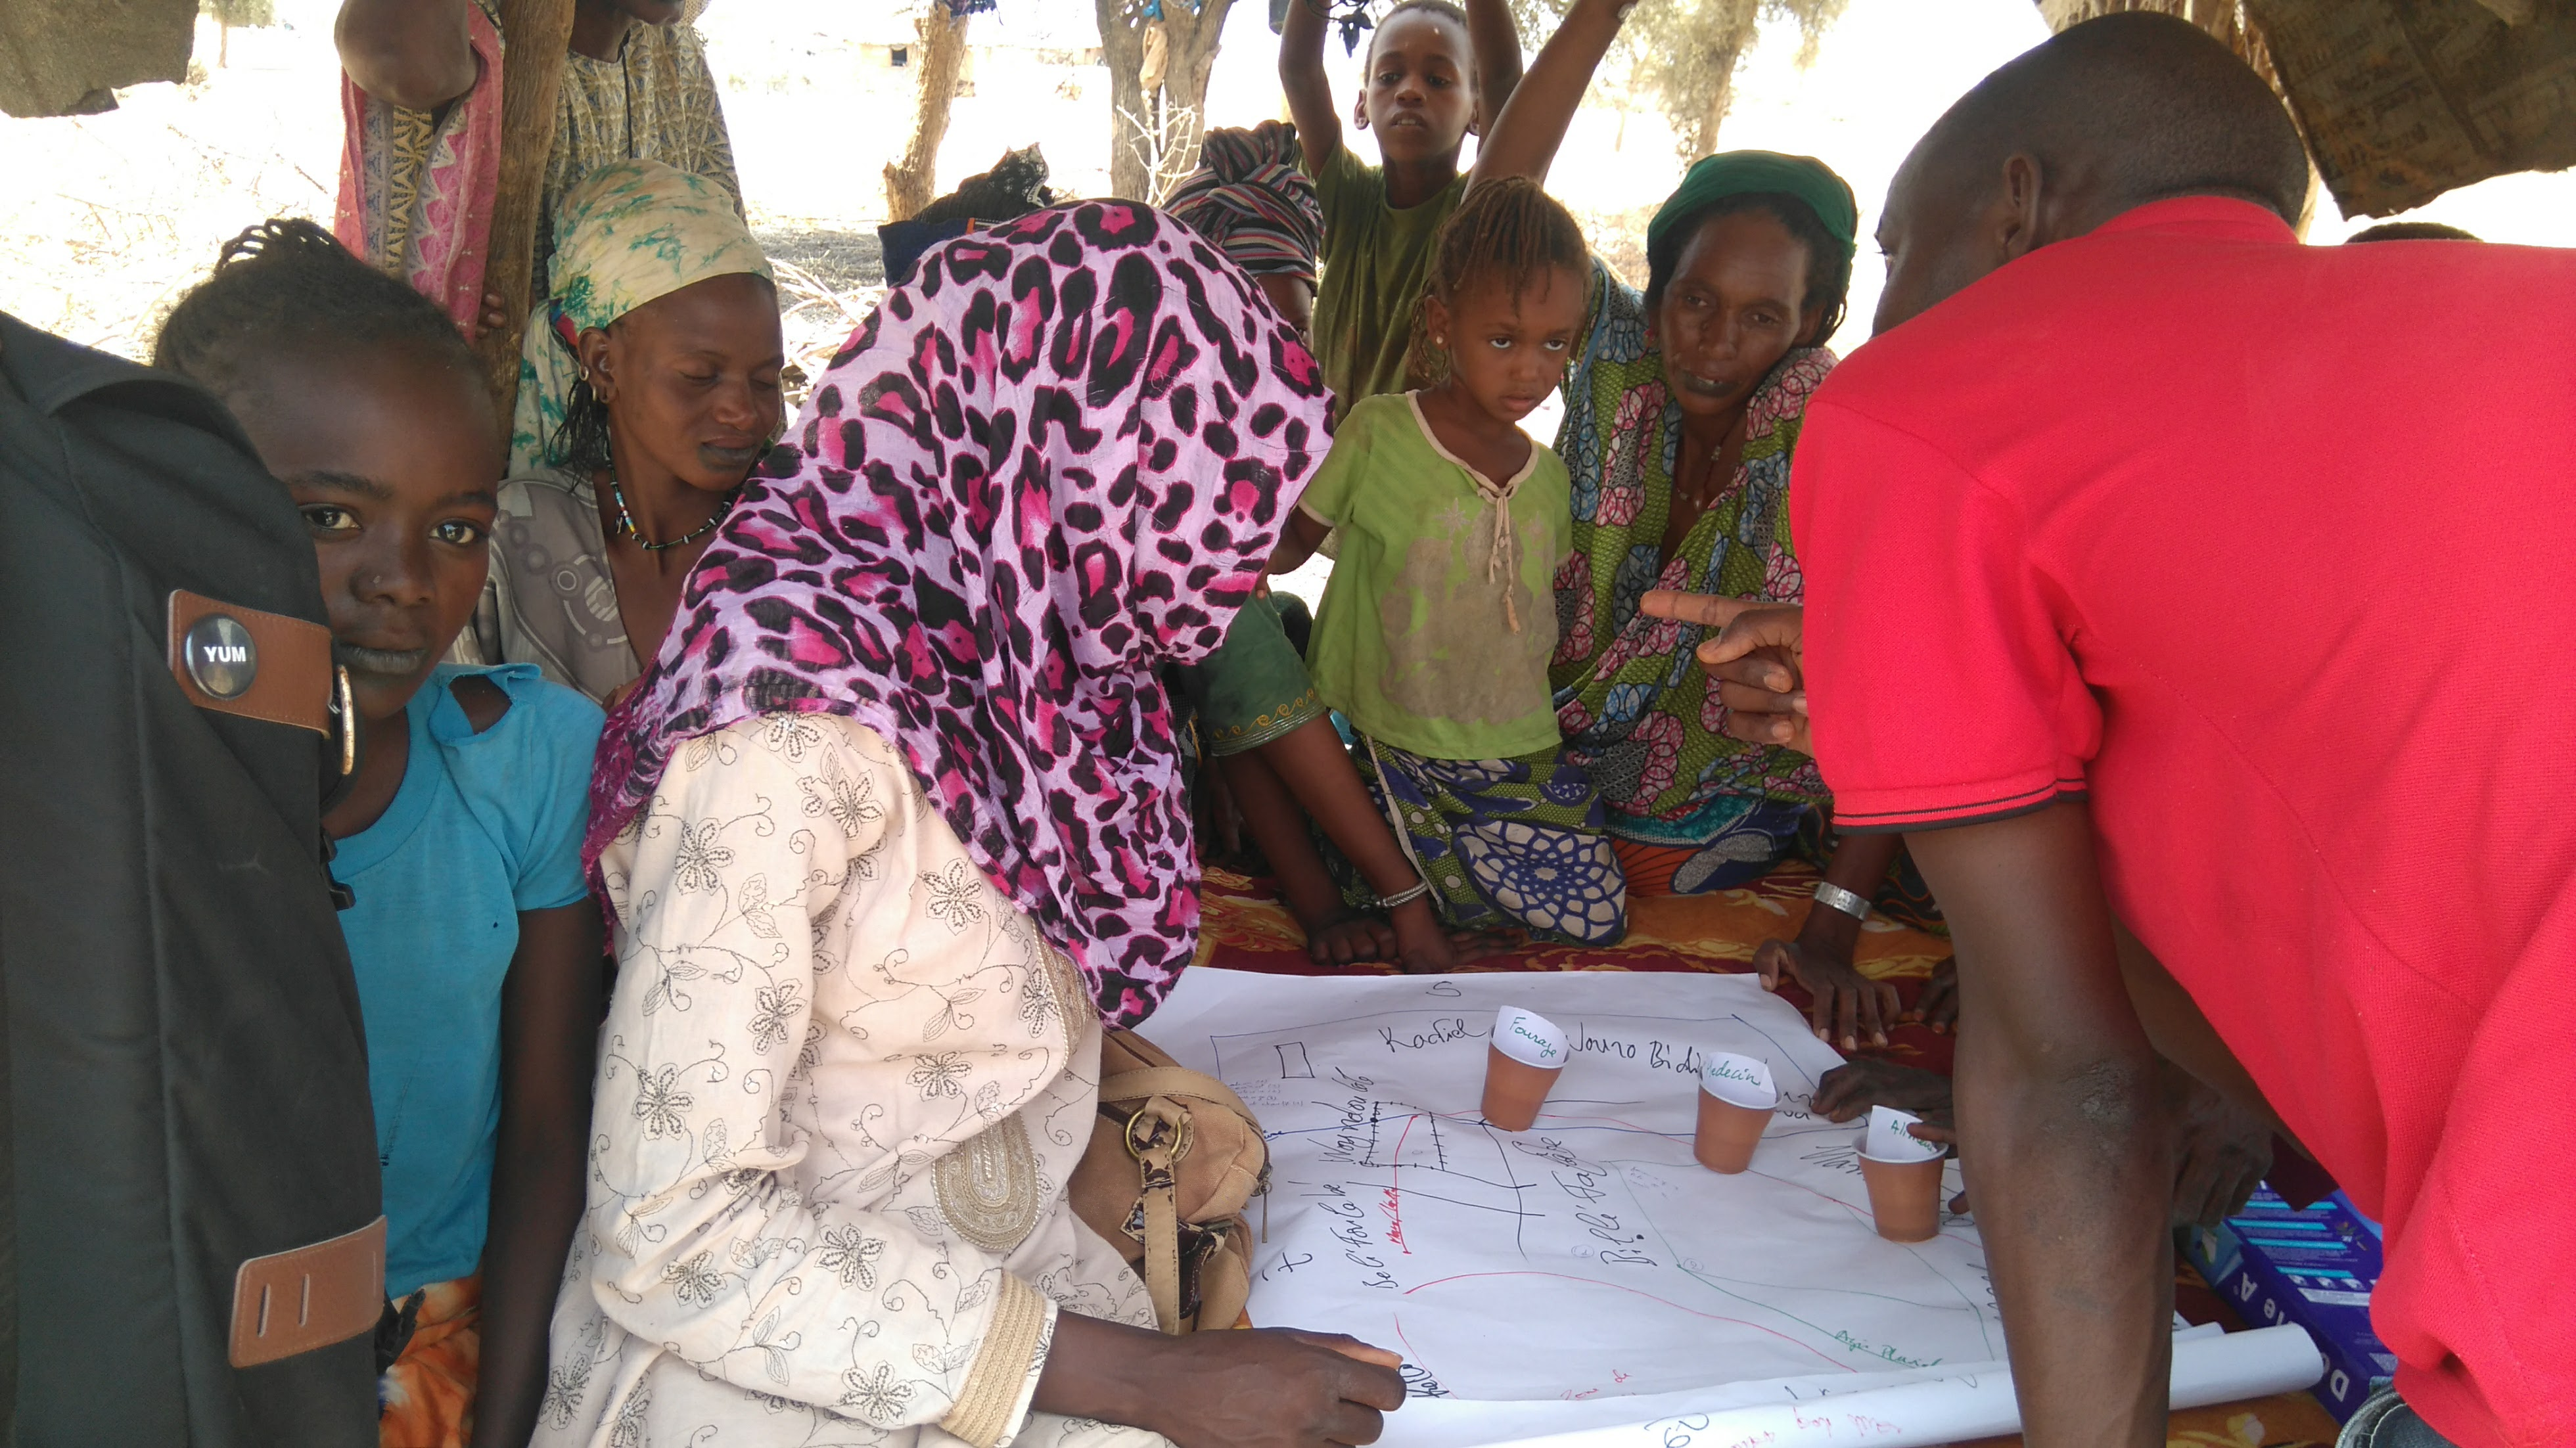
\includegraphics[width = 0.8\textwidth]{img/DSC_1793}
\end{figure}

\end{frame}

%-=-=-=-=-=-=-=-=-=-=-=-=-=-=-=-=-=-=-=-=-=-=-=-=
%	FRAME: Résultats
%-=-=-=-=-=-=-=-=-=-=-=-=-=-=-=-=-=-=-=-=-=-=-=-=

\section{Des premiers resultats}

\begin{frame}[c]{Résultat 1 : identification de "l'espace vécu"}
\vspace{-1cm}
\begin{figure}
	\subfigure[]{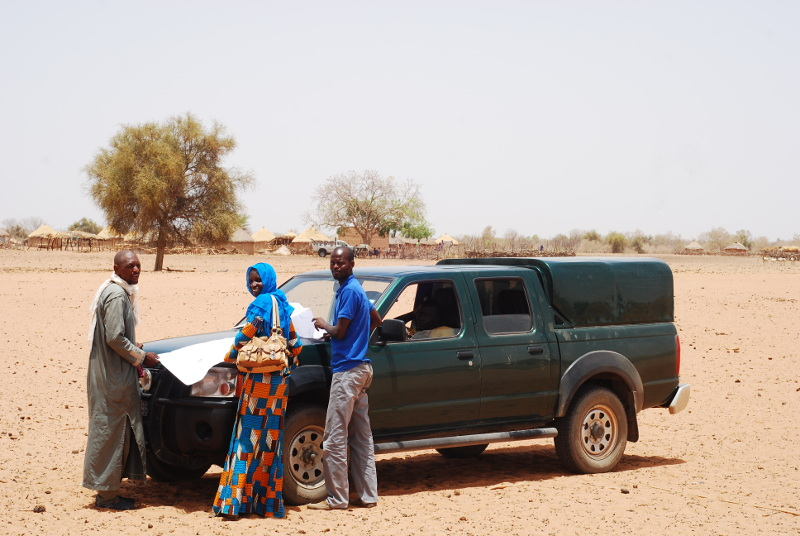
\includegraphics[height = 4.8cm]{img/DSC_0371}}
  \subfigure[]{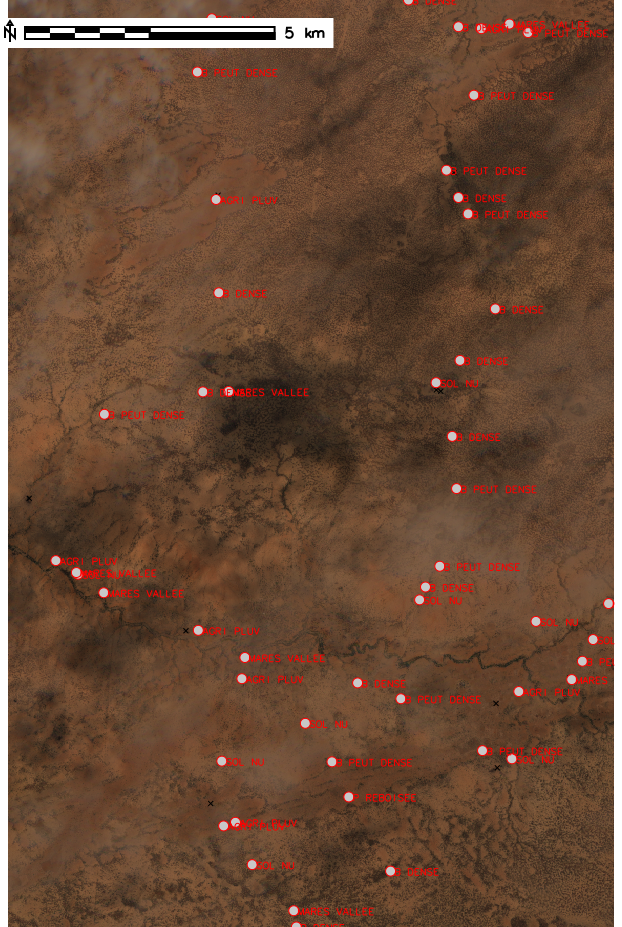
\includegraphics[height = 4.8cm]{img/map_RVB.png}}
\end{figure}
\end{frame}

%-=-=-=-=-=-=-=-=-=-=-=-=-=-=-=-=-=-=-=-=-=-=-=-=
%	FRAME: Classification
%-=-=-=-=-=-=-=-=-=-=-=-=-=-=-=-=-=-=-=-=-=-=-=-=
\begin{frame}[c]{Résultat 2 : Classification des patches}
\vspace{-1cm}
\begin{figure}
  \centering
  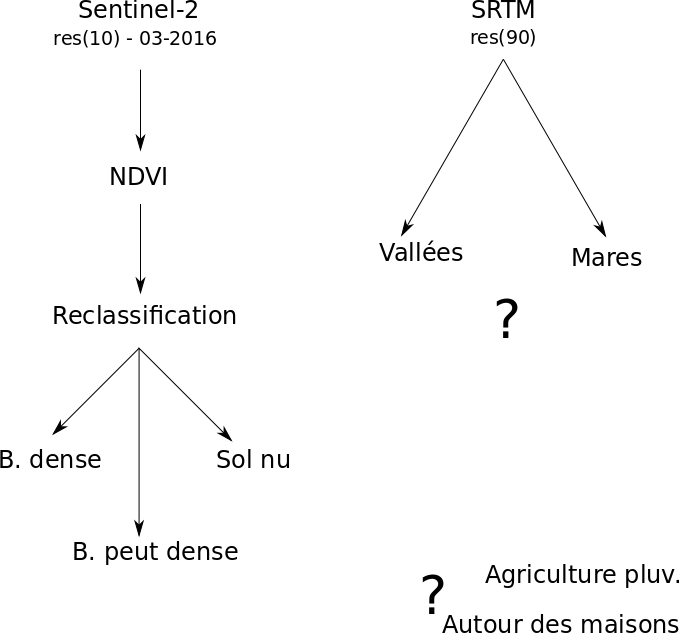
\includegraphics[width = 0.8\textwidth]{img/process}
\end{figure}

\end{frame}

\begin{frame}[c]{Résultat 2 : Classification des patches}
\vspace{-1cm}
\begin{figure}
	\subfigure[]{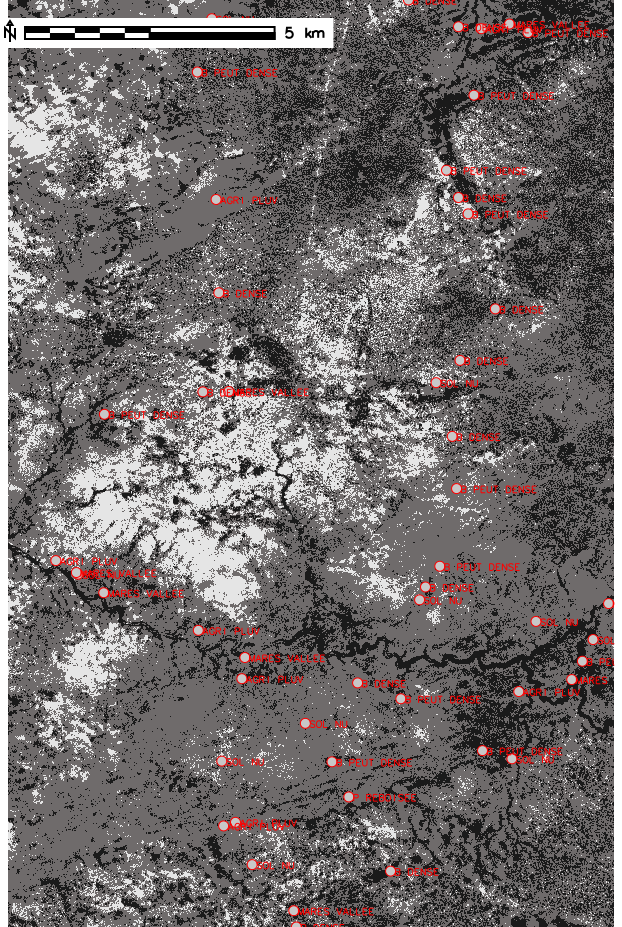
\includegraphics[height = 4.8cm]{img/map_classe_brousse}}
  \subfigure[]{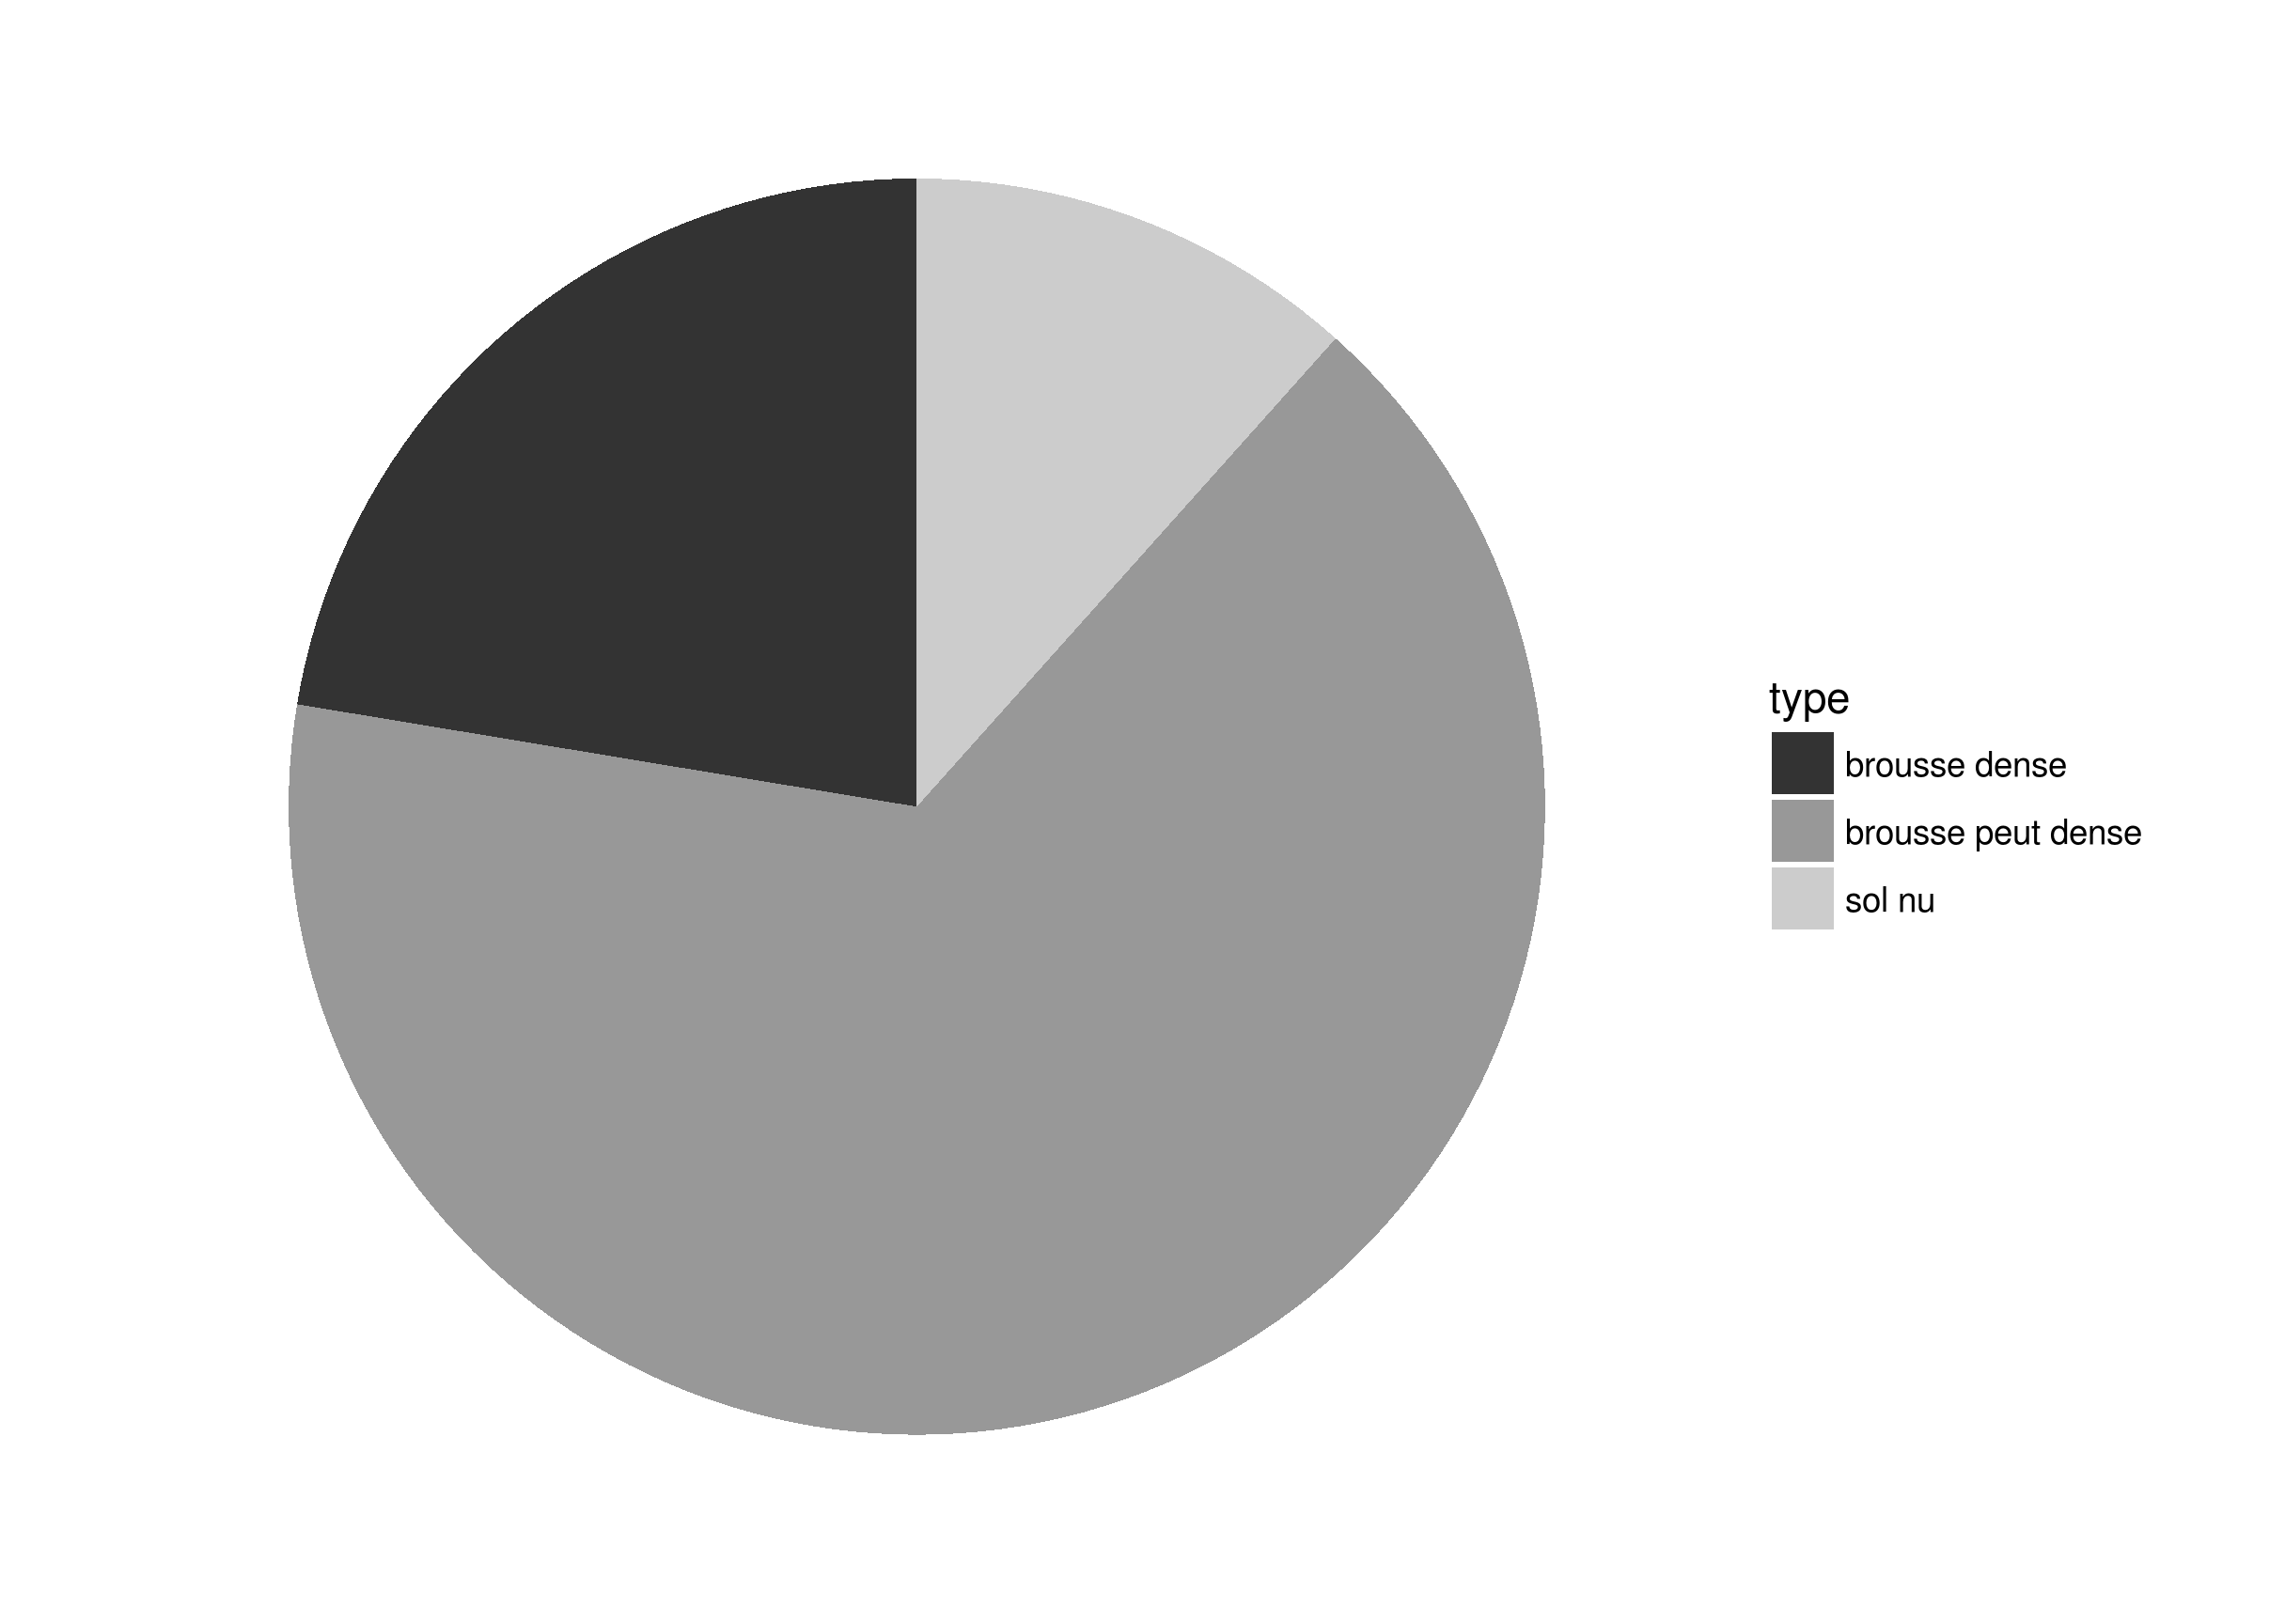
\includegraphics[height = 4.8cm]{img/pie_brousse}}
\end{figure}
\end{frame}

%-=-=-=-=-=-=-=-=-=-=-=-=-=-=-=-=-=-=-=-=-=-=-=-=
%	FRAME: Quantification
%-=-=-=-=-=-=-=-=-=-=-=-=-=-=-=-=-=-=-=-=-=-=-=-=
\begin{frame}[c]{Résultat 3 : Quantification}
\vspace{-1cm}
\begin{figure}
  \centering
  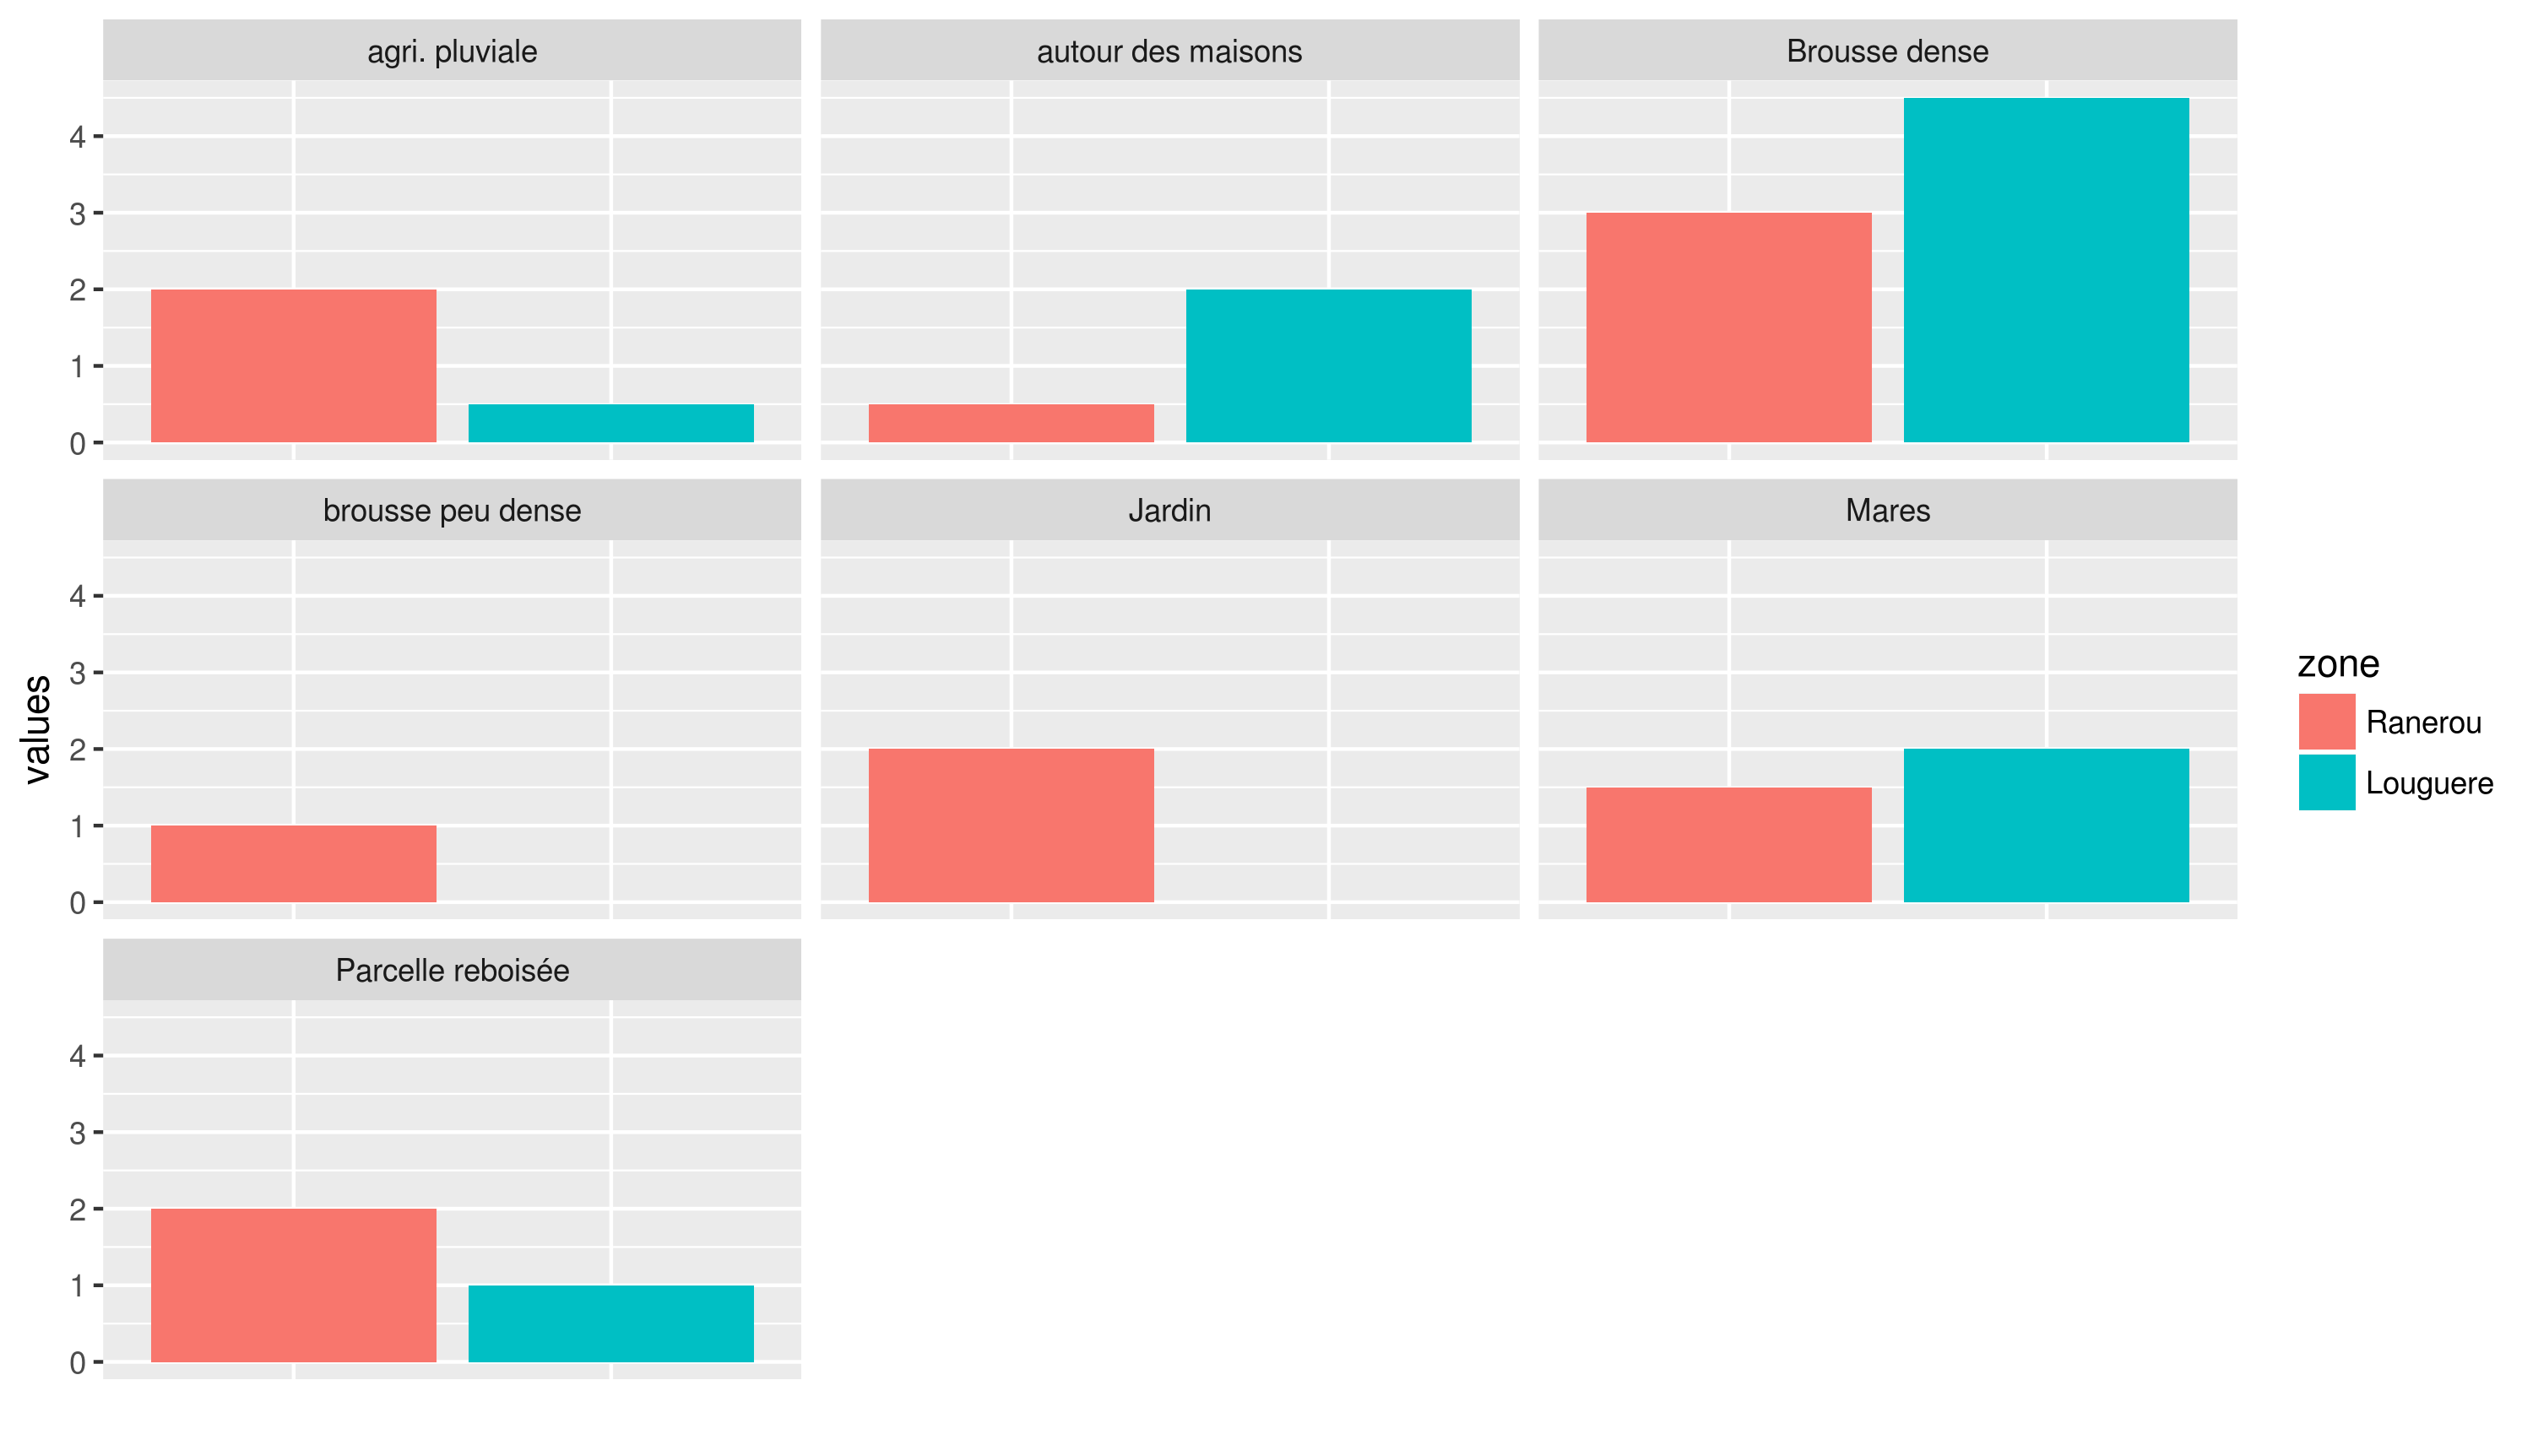
\includegraphics[width = \textwidth]{img/bar_general}
  \caption{La place de l'arbre vécu par unité spatiale}
\end{figure}

\end{frame}

\begin{frame}[c]{Résultat 3 : Quantification}
\vspace{-1cm}
\begin{figure}
  \centering
  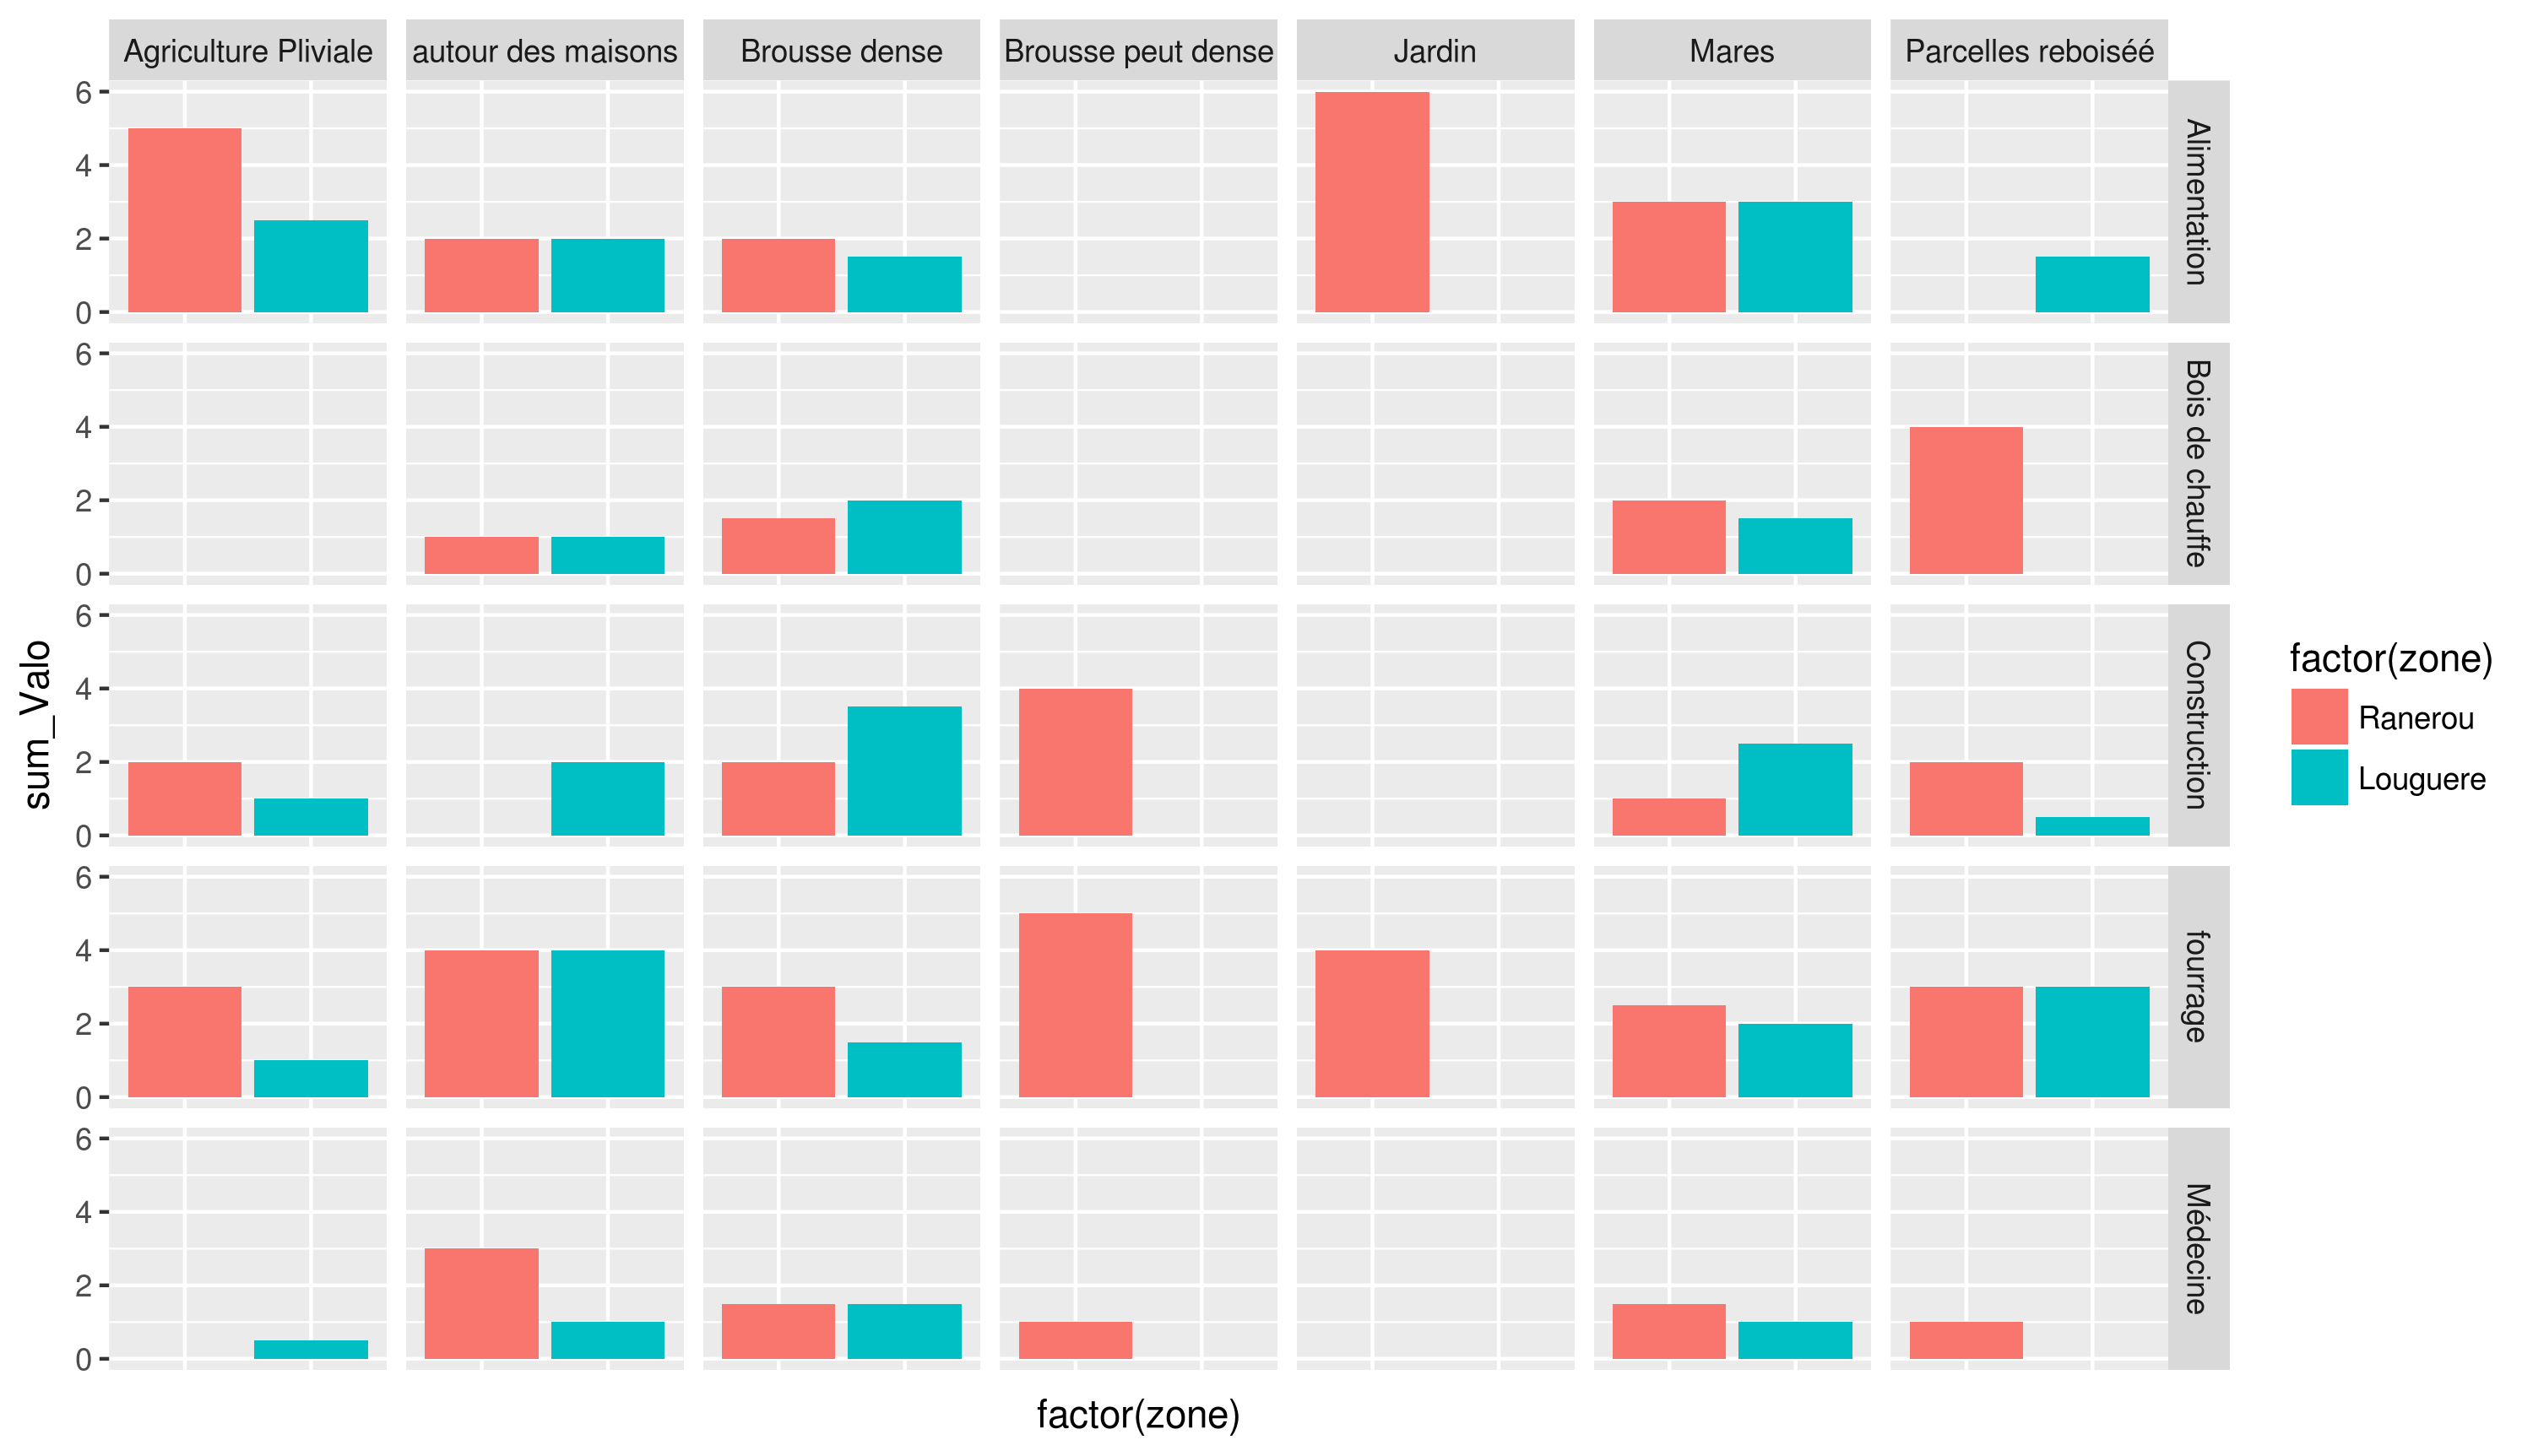
\includegraphics[width = \textwidth]{img/bar_se}
  \caption{Usage de l'arbre par unité spatiale}
\end{figure}

\end{frame}


%-=-=-=-=-=-=-=-=-=-=-=-=-=-=-=-=-=-=-=-=-=-=-=-=
%	FRAME: Conclusion
%-=-=-=-=-=-=-=-=-=-=-=-=-=-=-=-=-=-=-=-=-=-=-=-=
\section{Conclusion}
%-=-=-=-=-=-=-=-=-=-=-=-=-=-=-=-=-=-=-=-=-=-=-=-=
%	FRAME: Intégration à ComMod
%-=-=-=-=-=-=-=-=-=-=-=-=-=-=-=-=-=-=-=-=-=-=-=-=
\begin{frame}[c]{De l'arbre à la démarche ComMod}
\vspace{-1cm}
Une approche interdisciplinaire :
\begin{itemize}
  \item le travail d'enquête ethnobotanique permet d'identifier des pratiques socio-spatiales
  \item couplé au travail d'écologie du paysage, on identifie spatialement la contribution des lieux aux pratiques des habitants
  \item la formalisation des pratiques et de l'identification des lieux conduit à la formalisation de modèles de comportement et donc à une approche prospective validée par les acteurs.
\end{itemize}
\end{frame}


%-=-=-=-=-=-=-=-=-=-=-=-=-=-=-=-=-=-=-=-=-=-=-=-=
%	FRAME: MERCI DE VOTRE ATTENTION
%-=-=-=-=-=-=-=-=-=-=-=-=-=-=-=-=-=-=-=-=-=-=-=-=
{
\usebackgroundtemplate{
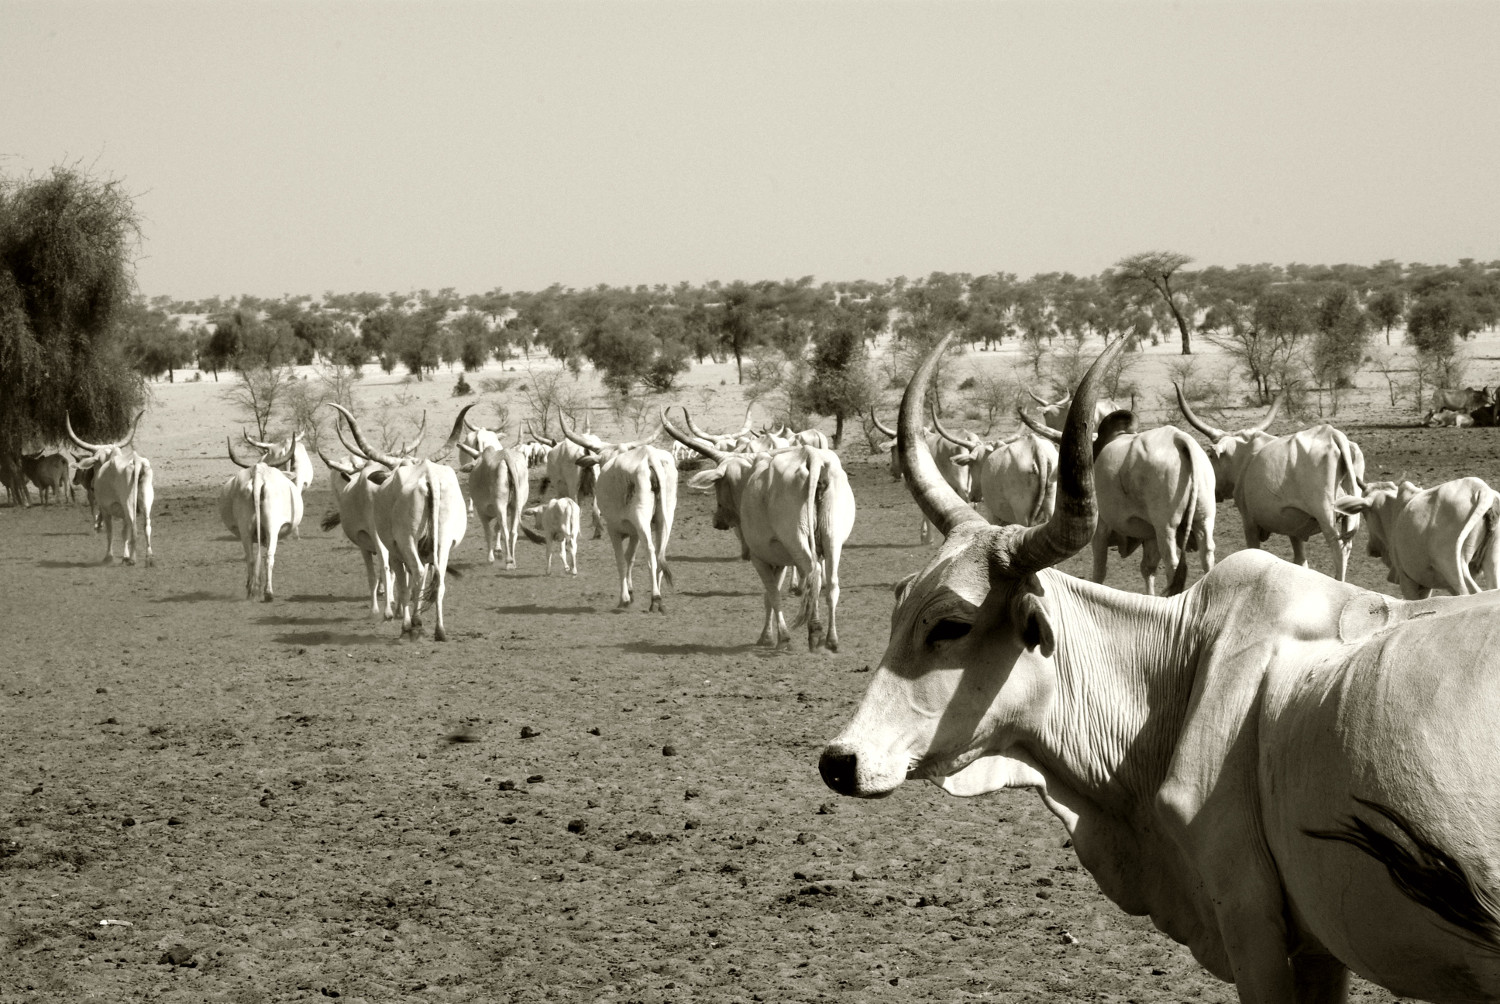
\includegraphics[width=\paperwidth]{img/podor_fin}}%
\begin{frame}
  \vspace{-1em}
  \begin{minipage}[t][.8\textheight]{\textwidth}
    \color{\cnGrey}{\LARGE{Thank you for your attention}}

    \vfill

  %\hfill \small{Photo credit : Thomas m-louis. sur \includegraphics[height=0.55cm]{img/flickr_logo}}
  \end{minipage}
  \vspace{-3.5em}
  \centering
	You can find this presentation on github
\includegraphics[height=0.85cm]{img/github}

\end{frame}
}


\end{document}
